\subsection{Normalización de datos}

\subsubsection{Normalización min-max}
La Figuras \ref{Fig: age_at_ercp_NORM} - \ref{Fig: cystic_duct_filling_NORM} muestran los resultados de normalización de los atributos elegidos para el método min-max.

\begin{figure}[!htb]
	\centering
	\begin{subfigure}[b]{0.4\textwidth}
		\centering
		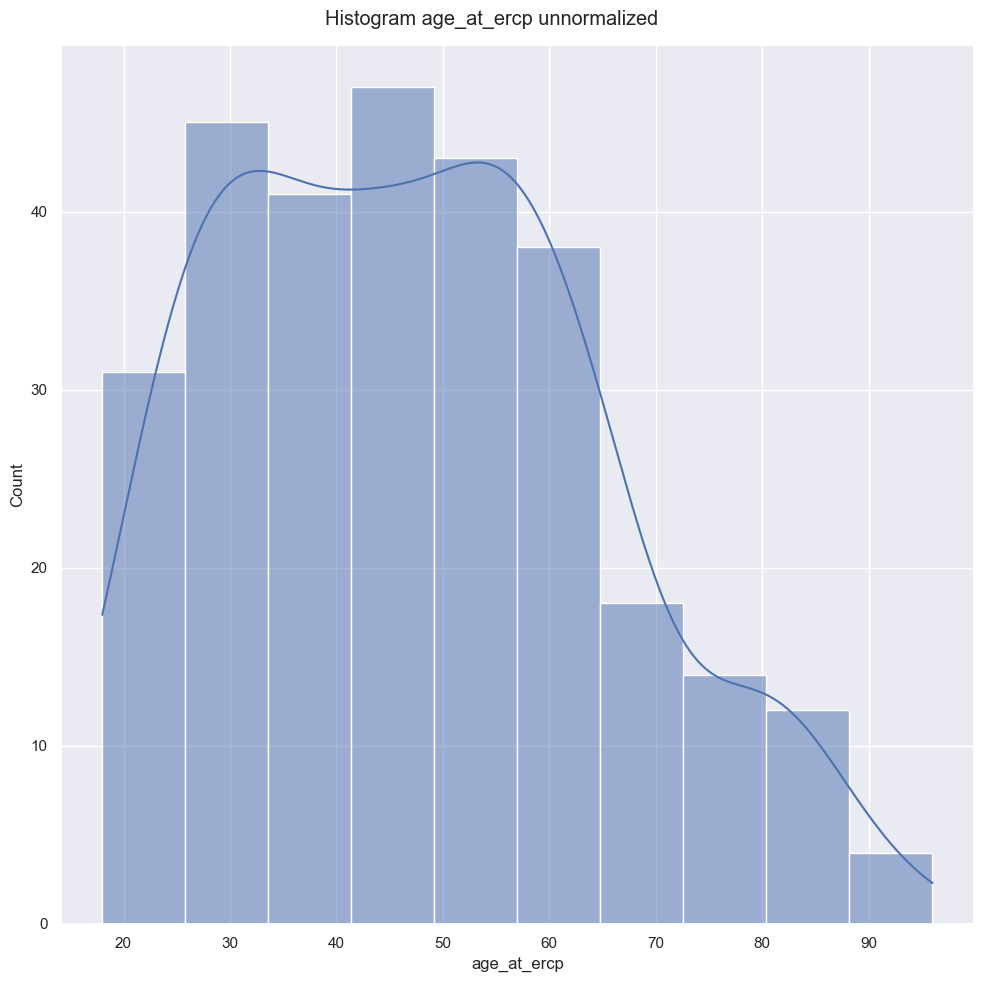
\includegraphics[width=\textwidth]{histogram_age_at_ercp_unnormalized}
		\caption{Histograma de atributo \emph{age\_at\_ercp} sin normalizar.}
	\end{subfigure}
	\hfill
	\begin{subfigure}[b]{0.4\textwidth}
		\centering
		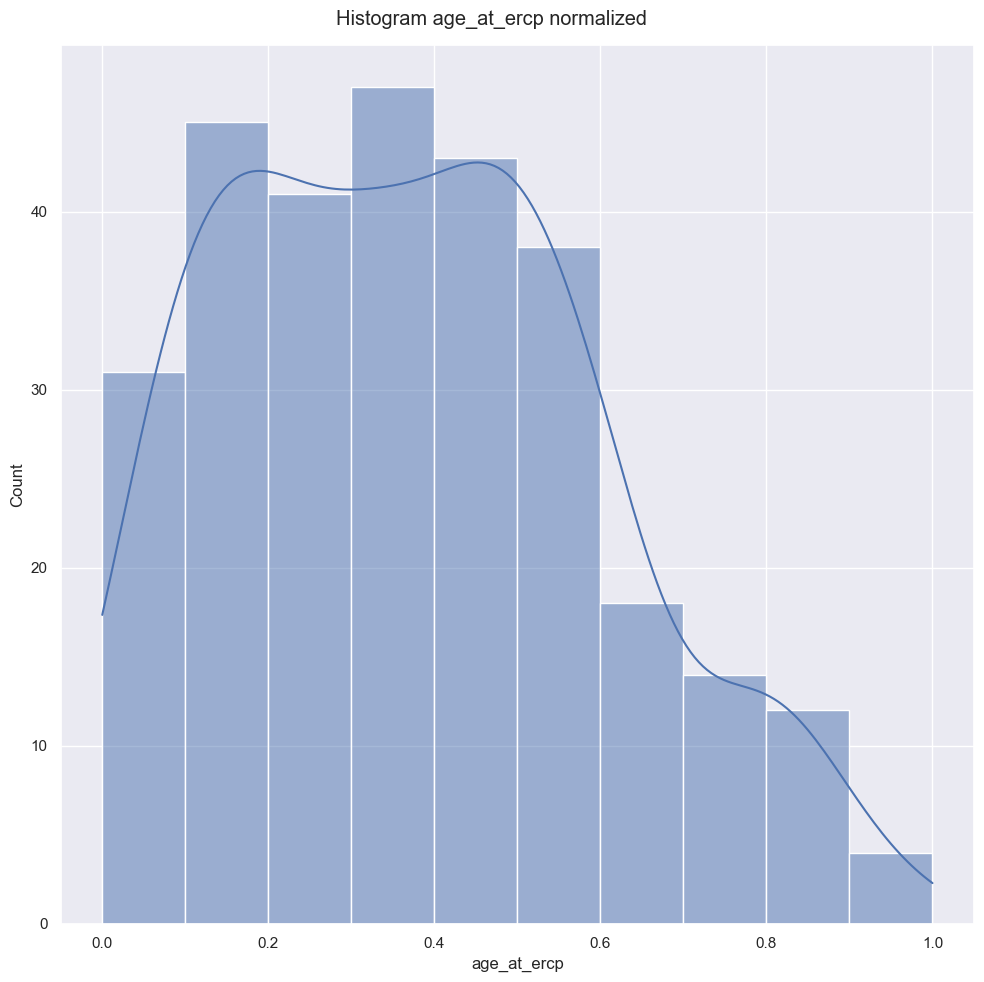
\includegraphics[width=\textwidth]{histogram_age_at_ercp_normalized}
		\caption{Histograma de atributo \emph{age\_at\_ercp} posterior a normalización.}
	\end{subfigure}
	\caption{Resultados de normalización de atributo \emph{age\_at\_ercp}}
	\label{Fig: age_at_ercp_NORM}
\end{figure}


\begin{figure}[!htb]
	\centering
	\begin{subfigure}[b]{0.4\textwidth}
		\centering
		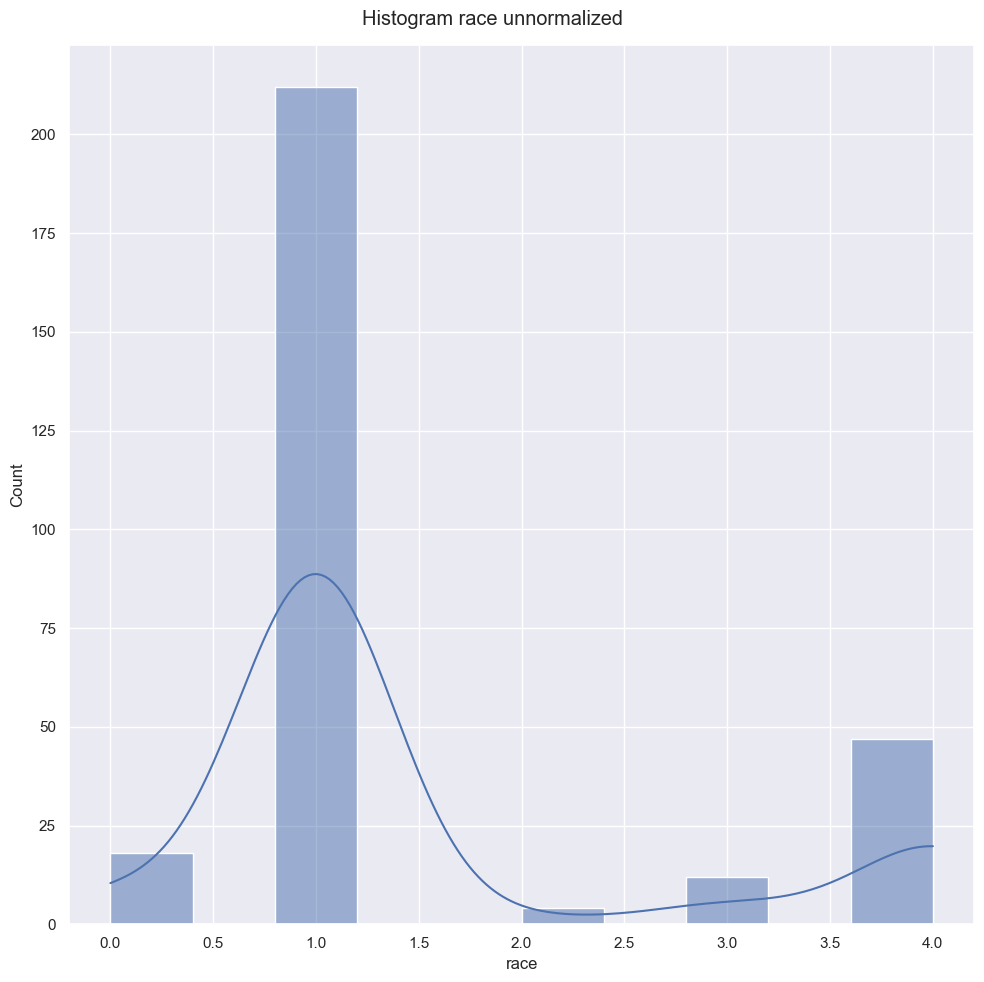
\includegraphics[width=\textwidth]{histogram_race_unnormalized}
		\caption{Histograma de atributo \emph{race} sin normalizar.}
	\end{subfigure}
	\hfill
	\begin{subfigure}[b]{0.4\textwidth}
		\centering
		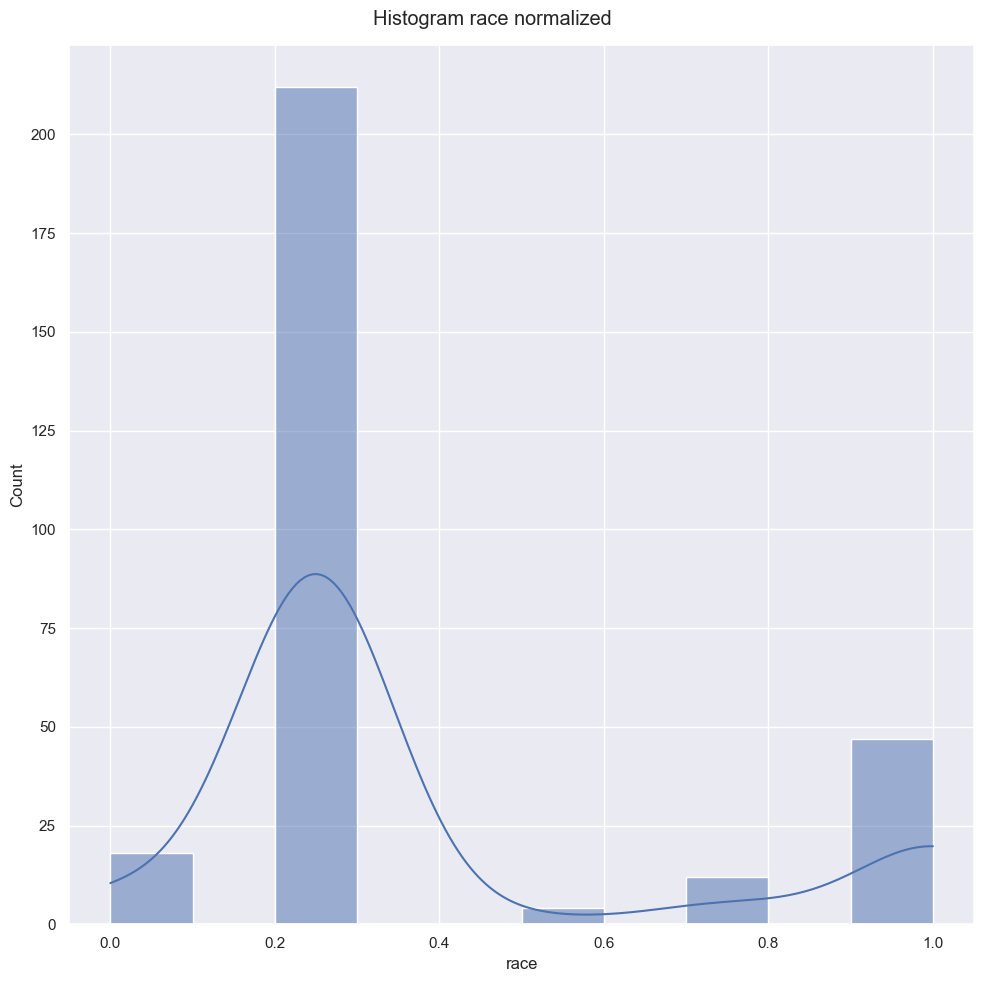
\includegraphics[width=\textwidth]{histogram_race_normalized}
		\caption{Histograma de atributo \emph{race} posterior a normalización.}
	\end{subfigure}
	\caption{Resultados de normalización de atributo \emph{race}}
	\label{Fig: race_NORM}
\end{figure}


\begin{figure}[!htb]
	\centering
	\begin{subfigure}[b]{0.4\textwidth}
		\centering
		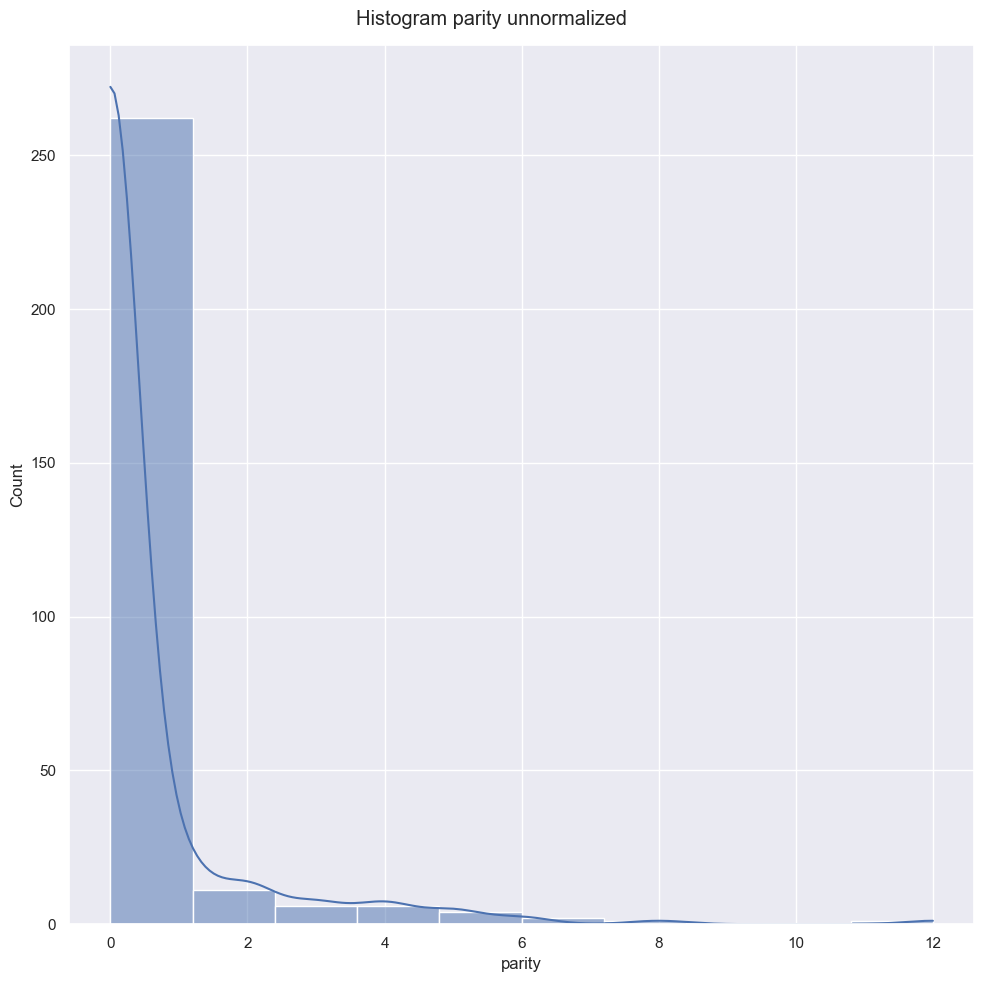
\includegraphics[width=\textwidth]{histogram_parity_unnormalized}
		\caption{Histograma de atributo \emph{parity} sin normalizar.}
	\end{subfigure}
	\hfill
	\begin{subfigure}[b]{0.4\textwidth}
		\centering
		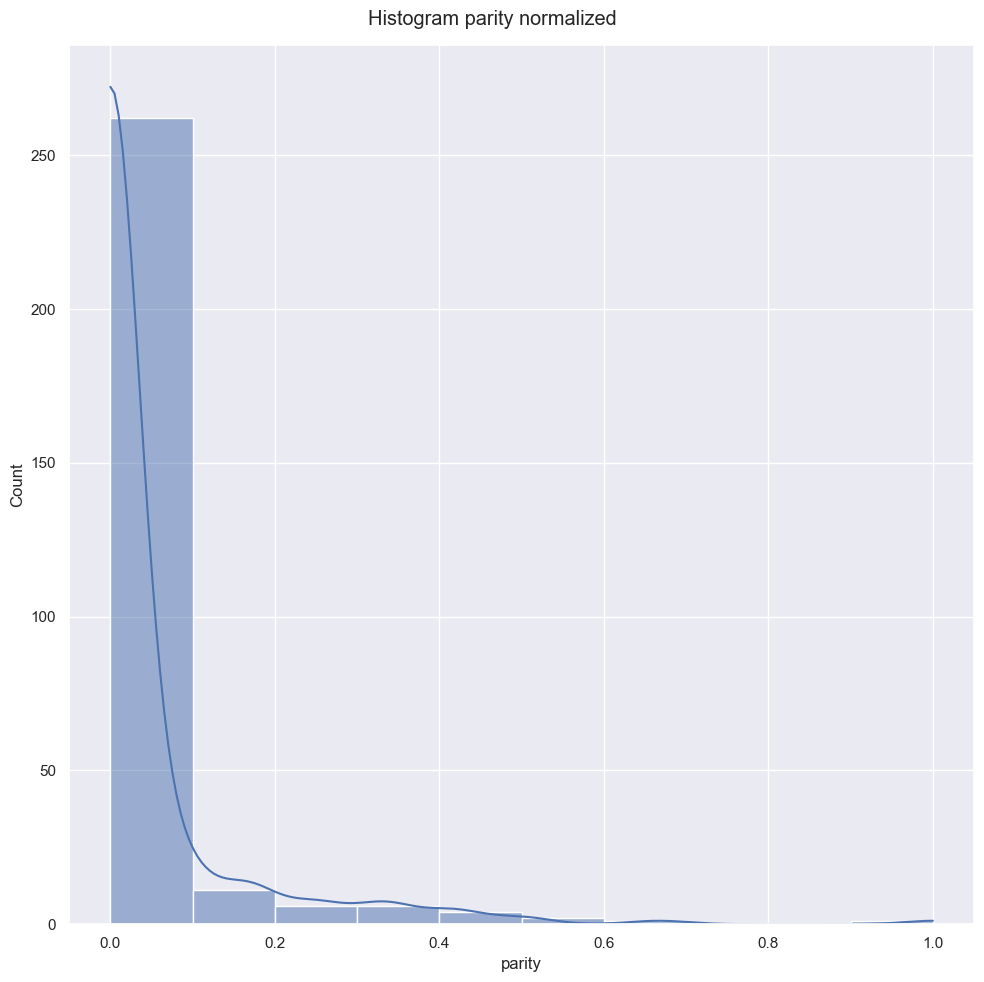
\includegraphics[width=\textwidth]{histogram_parity_normalized}
		\caption{Histograma de atributo \emph{parity} posterior a normalización.}
	\end{subfigure}
	\caption{Resultados de normalización de atributo \emph{parity}}
	\label{Fig: parity_NORM}
\end{figure}


\begin{figure}[!htb]
	\centering
	\begin{subfigure}[b]{0.4\textwidth}
		\centering
		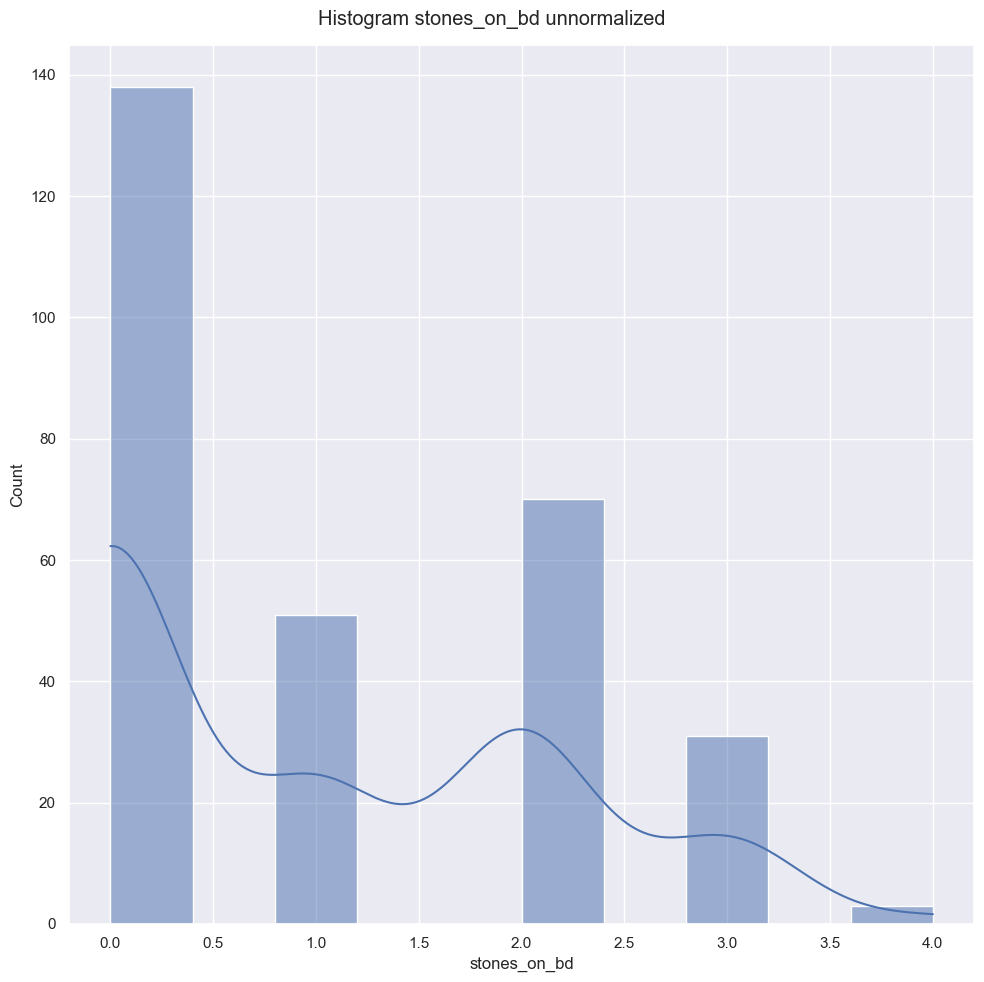
\includegraphics[width=\textwidth]{histogram_stones_on_bd_unnormalized}
		\caption{Histograma de atributo \emph{stones\_on\_bd} sin normalizar.}
	\end{subfigure}
	\hfill
	\begin{subfigure}[b]{0.4\textwidth}
		\centering
		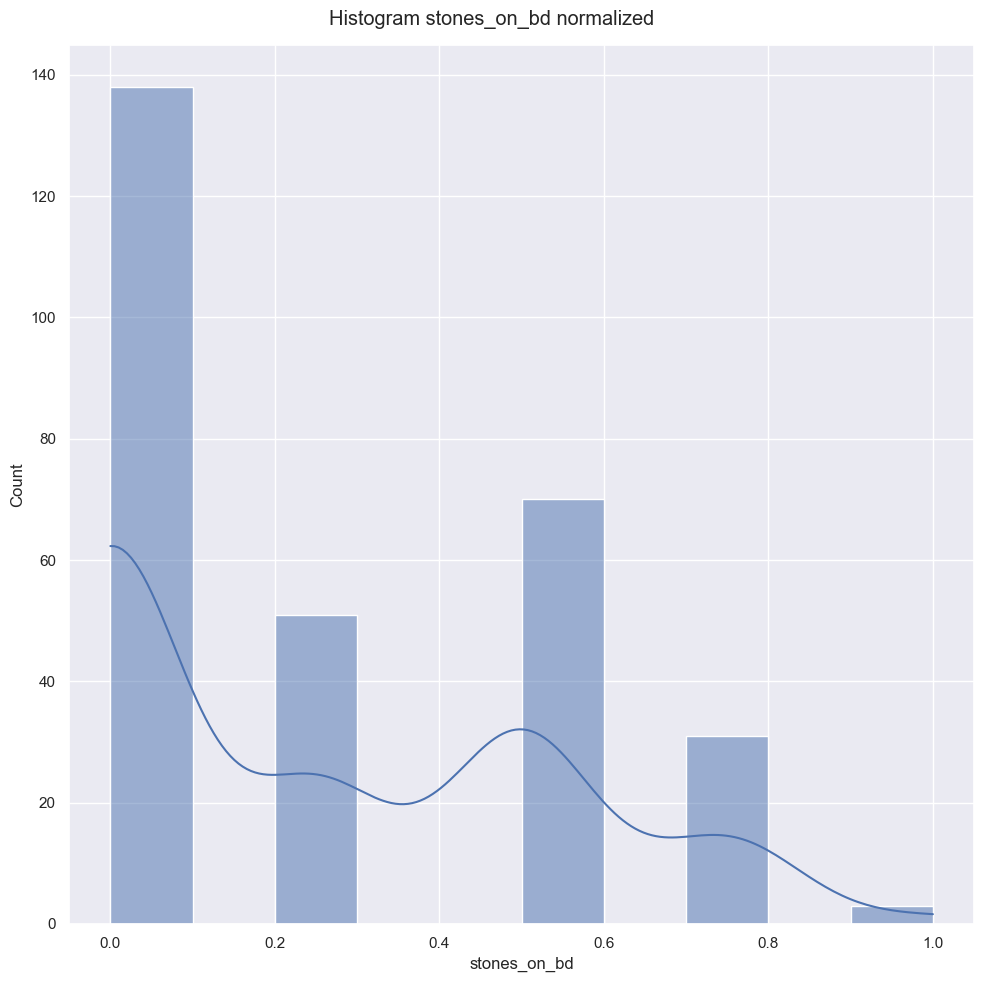
\includegraphics[width=\textwidth]{histogram_stones_on_bd_normalized}
		\caption{Histograma de atributo \emph{stones\_on\_bd} posterior a normalización.}
	\end{subfigure}
	\caption{Resultados de normalización de atributo \emph{stones\_on\_bd}}
	\label{Fig: stones_on_bd_NORM}
\end{figure}


\begin{figure}[!htb]
	\centering
	\begin{subfigure}[b]{0.4\textwidth}
		\centering
		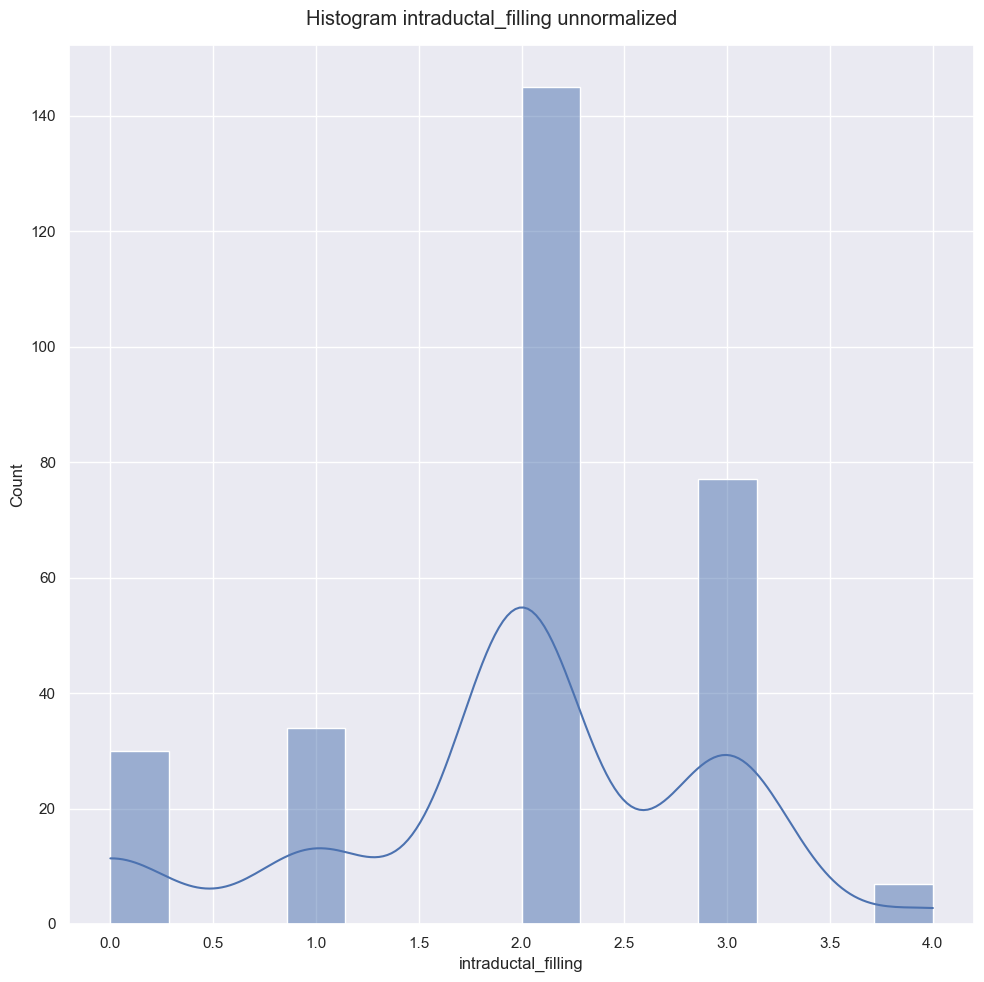
\includegraphics[width=\textwidth]{histogram_intraductal_filling_unnormalized}
		\caption{Histograma de atributo \emph{intraductal\_filling} sin normalizar.}
	\end{subfigure}
	\hfill
	\begin{subfigure}[b]{0.4\textwidth}
		\centering
		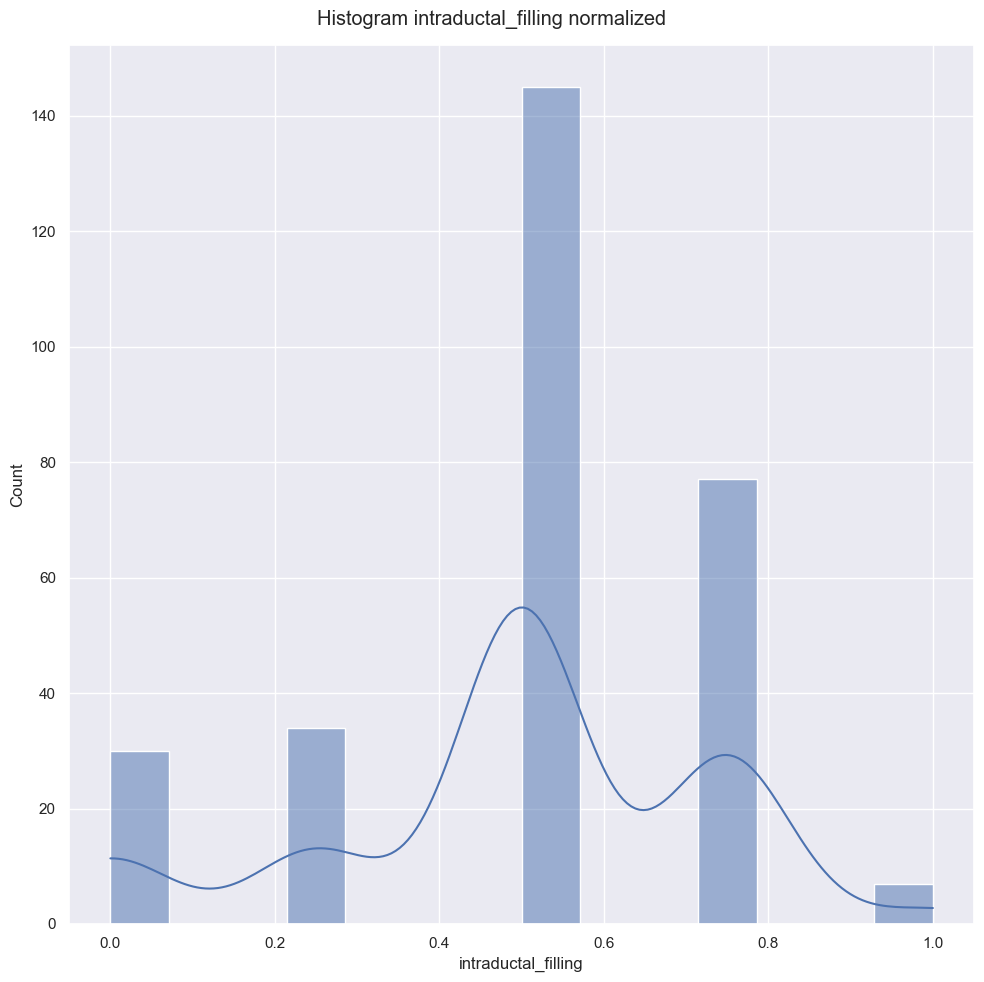
\includegraphics[width=\textwidth]{histogram_intraductal_filling_normalized}
		\caption{Histograma de atributo \emph{intraductal\_filling} posterior a normalización.}
	\end{subfigure}
	\caption{Resultados de normalización de atributo \emph{intraductal\_filling}}
	\label{Fig: intraductal_filling_NORM}
\end{figure}


\begin{figure}[!htb]
	\centering
	\begin{subfigure}[b]{0.4\textwidth}
		\centering
		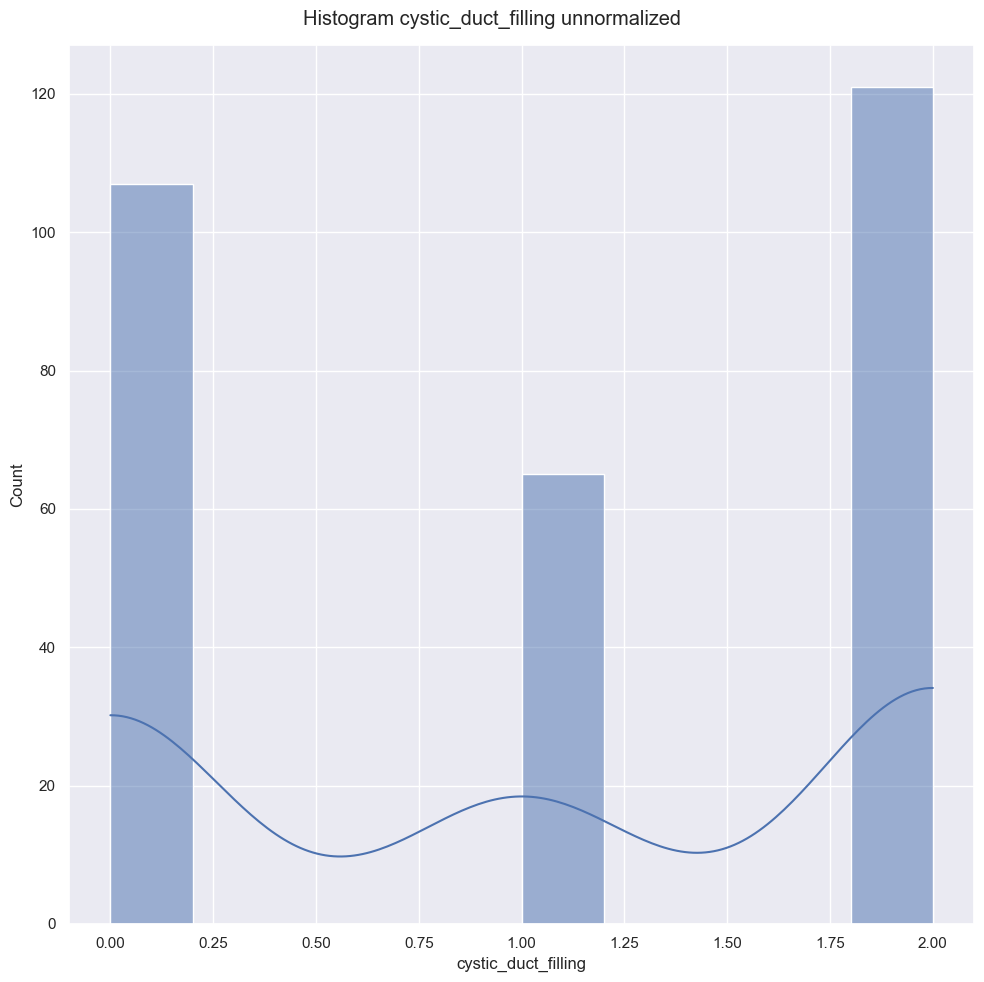
\includegraphics[width=\textwidth]{histogram_cystic_duct_filling_unnormalized}
		\caption{Histograma de atributo \emph{cystic\_duct\_filling} sin normalizar.}
	\end{subfigure}
	\hfill
	\begin{subfigure}[b]{0.4\textwidth}
		\centering
		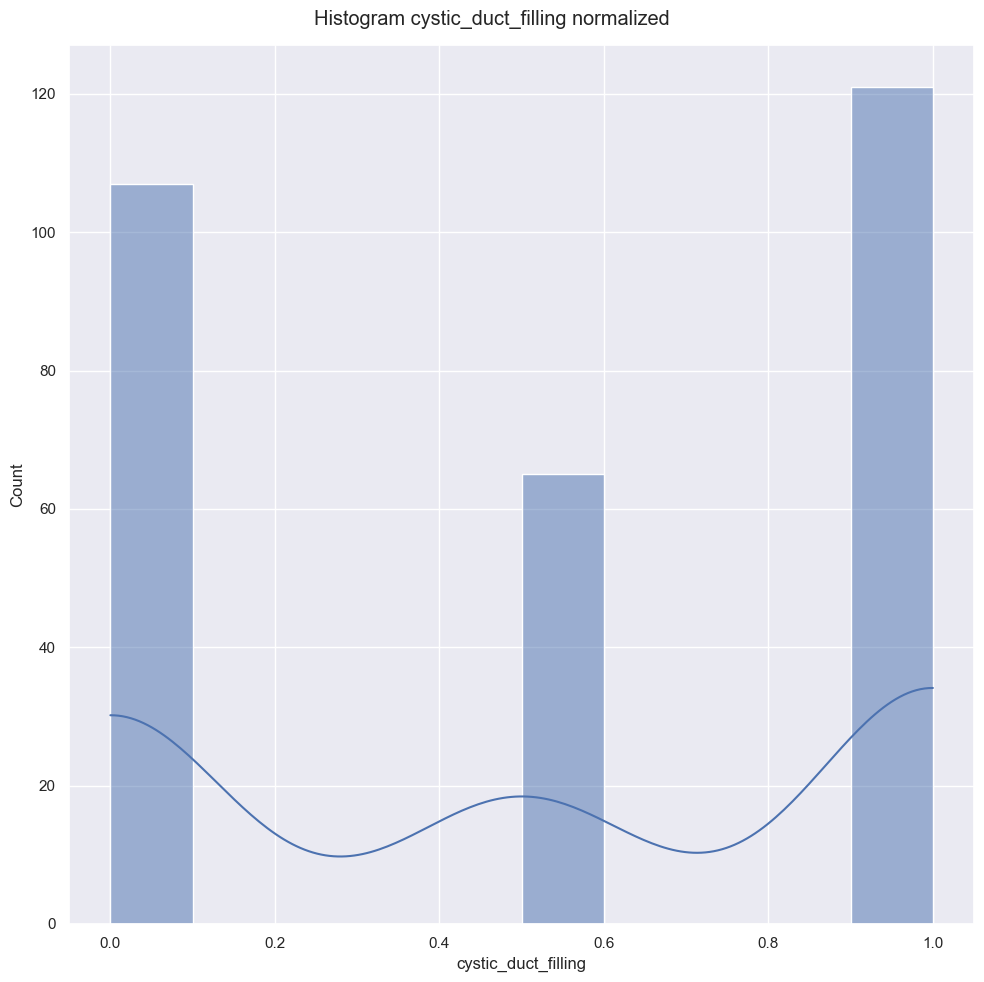
\includegraphics[width=\textwidth]{histogram_cystic_duct_filling_normalized}
		\caption{Histograma de atributo \emph{cystic\_duct\_filling} posterior a normalización.}
	\end{subfigure}
	\caption{Resultados de normalización de atributo \emph{cystic\_duct\_filling}}
	\label{Fig: cystic_duct_filling_NORM}
\end{figure}


\FloatBarrier
\subsubsection{Normalización z-score}
La Figuras \ref{Fig: bmi_NORM} - \ref{Fig: cbd_diameter_ercp_NORM} muestran los resultados de normalización de los atributos elegidos para el método z-score.

\begin{figure}[!htb]
	\centering
	\begin{subfigure}[b]{0.4\textwidth}
		\centering
		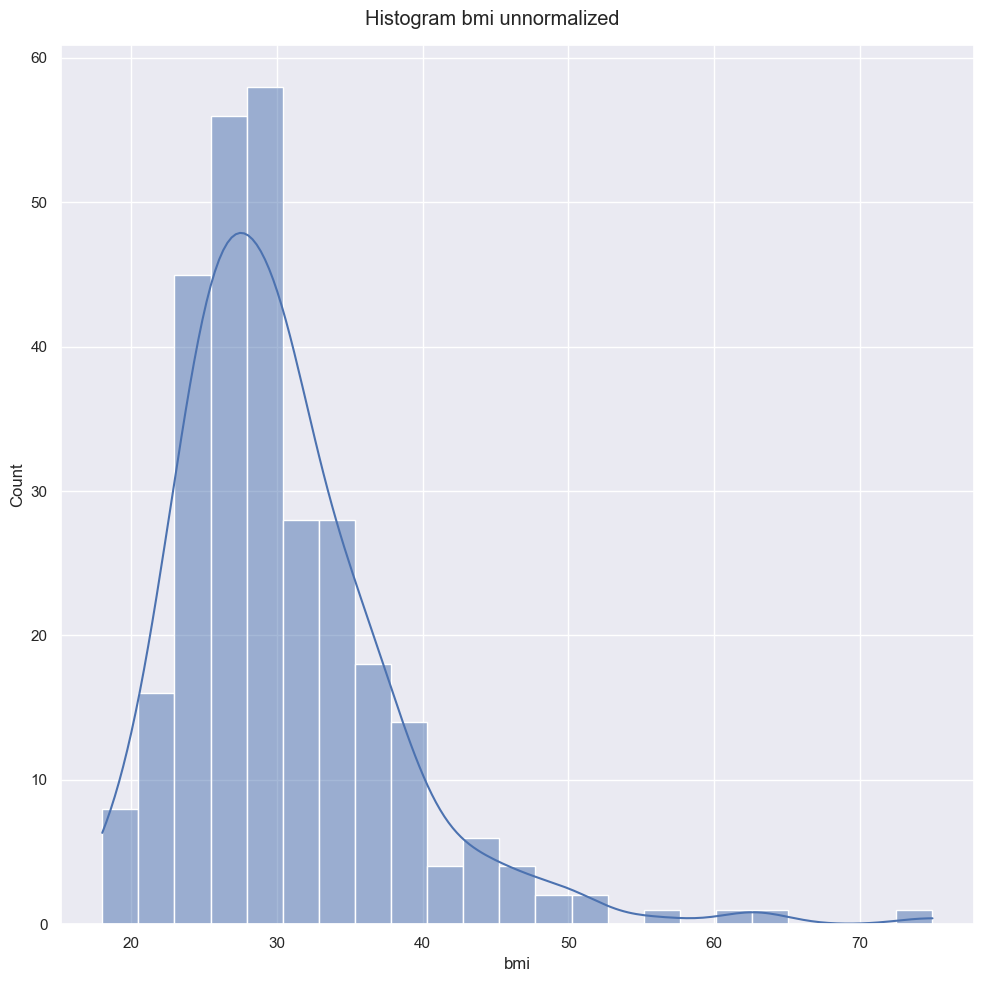
\includegraphics[width=\textwidth]{histogram_bmi_unnormalized}
		\caption{Histograma de atributo \emph{bmi} sin normalizar.}
	\end{subfigure}
	\hfill
	\begin{subfigure}[b]{0.4\textwidth}
		\centering
		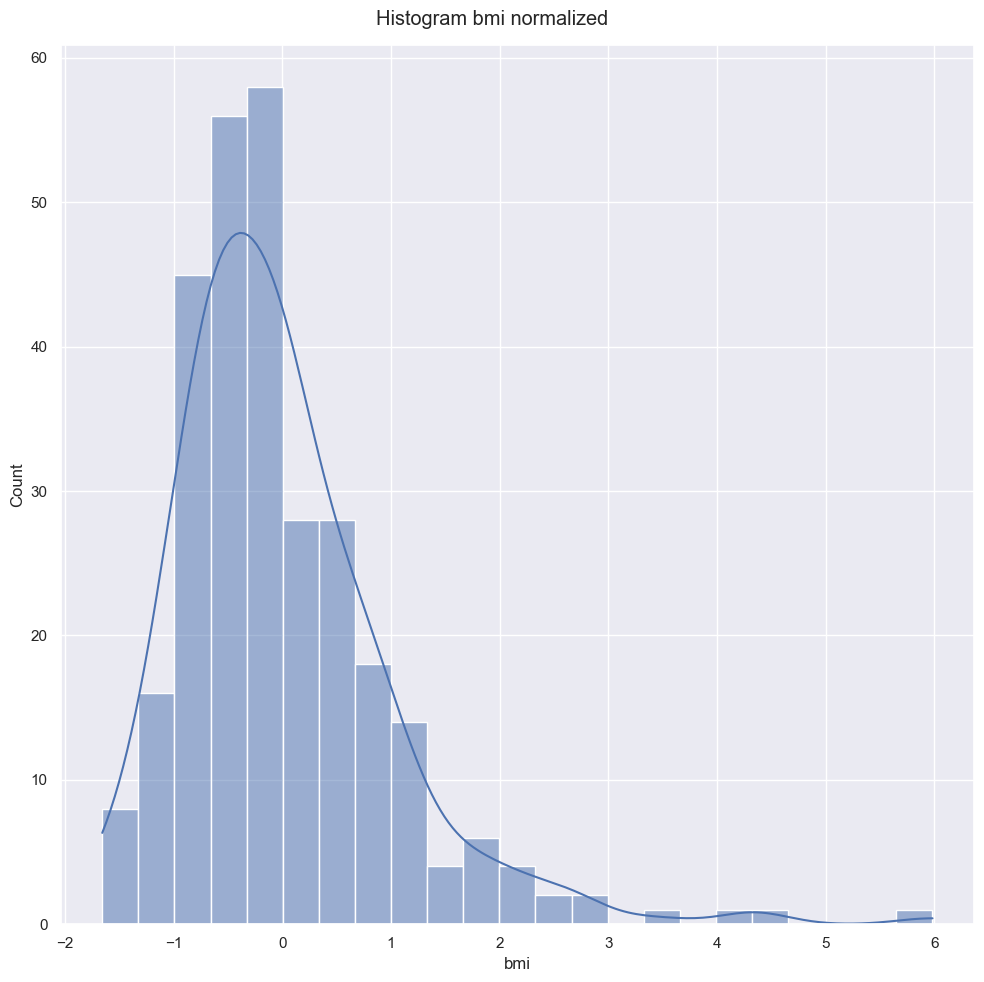
\includegraphics[width=\textwidth]{histogram_bmi_normalized}
		\caption{Histograma de atributo \emph{bmi} posterior a normalización.}
	\end{subfigure}
	\caption{Resultados de normalización de atributo \emph{bmi}}
	\label{Fig: bmi_NORM}
\end{figure}


\begin{figure}[!htb]
	\centering
	\begin{subfigure}[b]{0.4\textwidth}
		\centering
		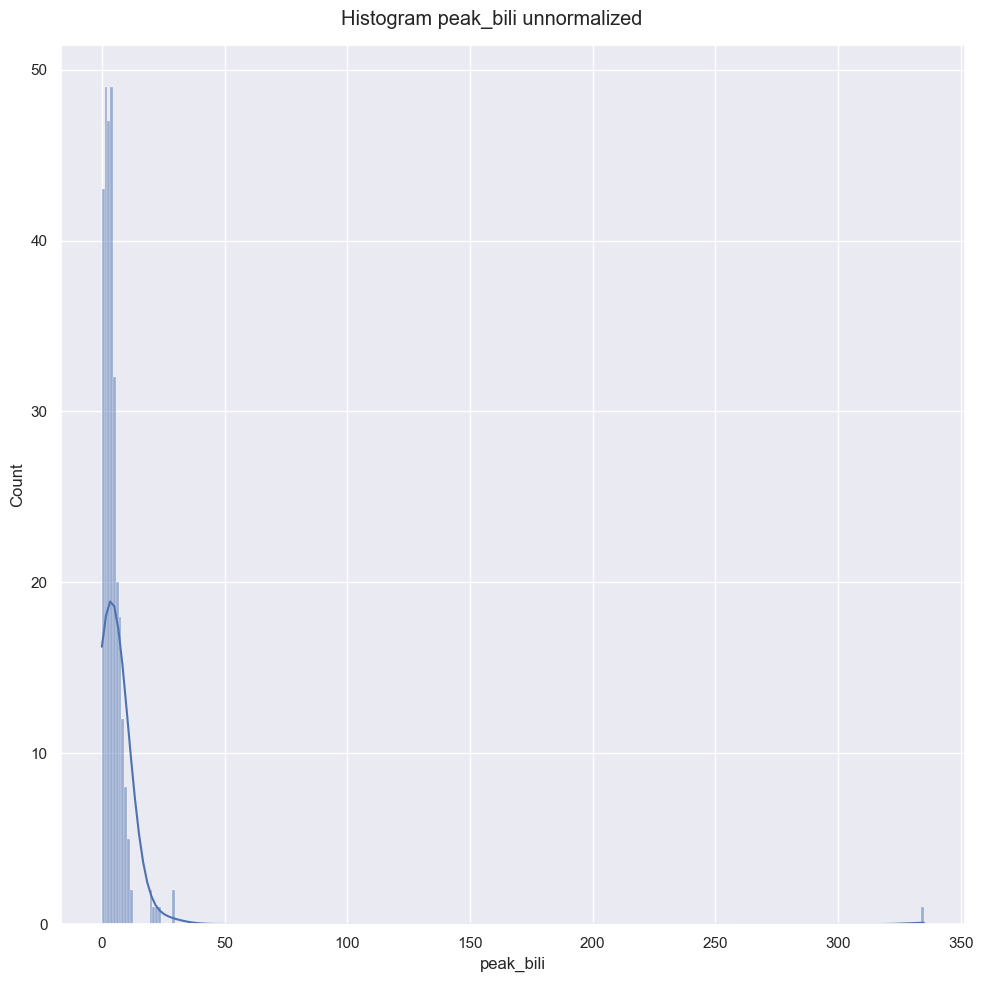
\includegraphics[width=\textwidth]{histogram_peak_bili_unnormalized}
		\caption{Histograma de atributo \emph{peak\_bili} sin normalizar.}
	\end{subfigure}
	\hfill
	\begin{subfigure}[b]{0.4\textwidth}
		\centering
		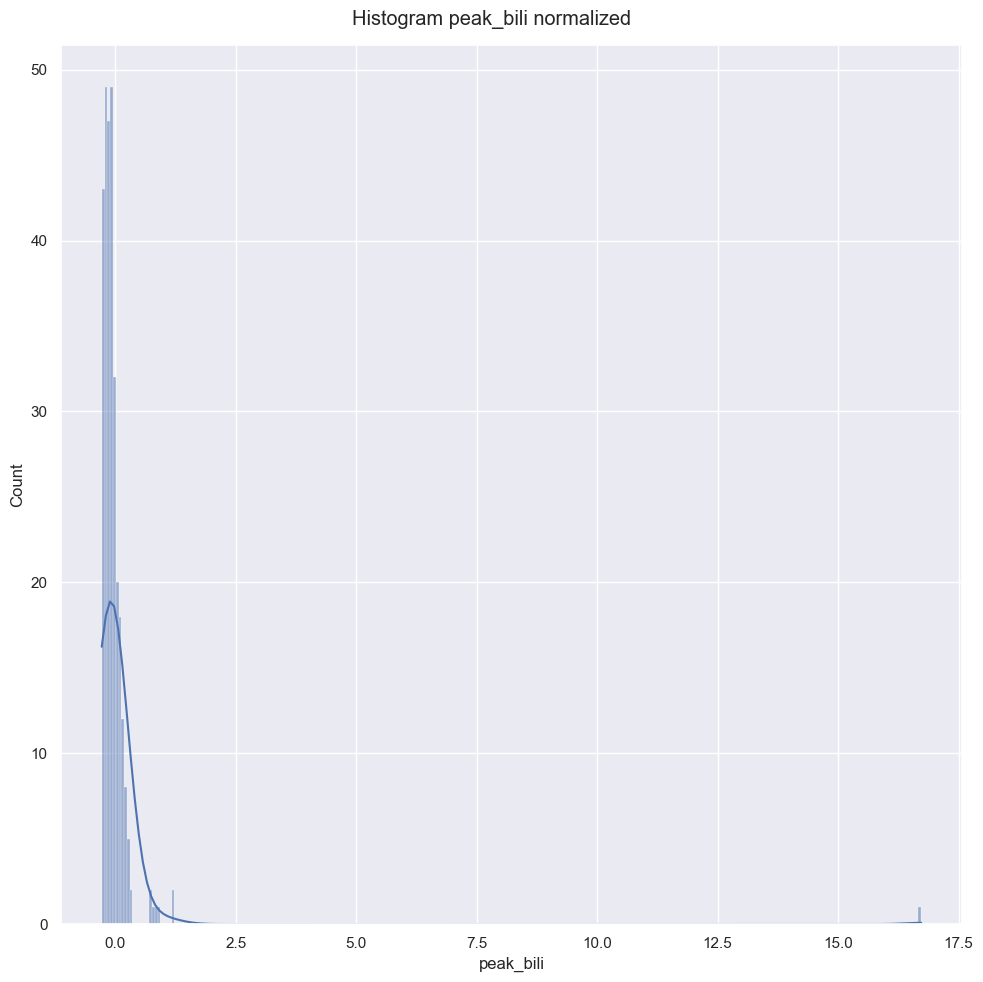
\includegraphics[width=\textwidth]{histogram_peak_bili_normalized}
		\caption{Histograma de atributo \emph{peak\_bili} posterior a normalización.}
	\end{subfigure}
	\caption{Resultados de normalización de atributo \emph{peak\_bili}}
	\label{Fig: peak_bili_NORM}
\end{figure}


\begin{figure}[!htb]
	\centering
	\begin{subfigure}[b]{0.4\textwidth}
		\centering
		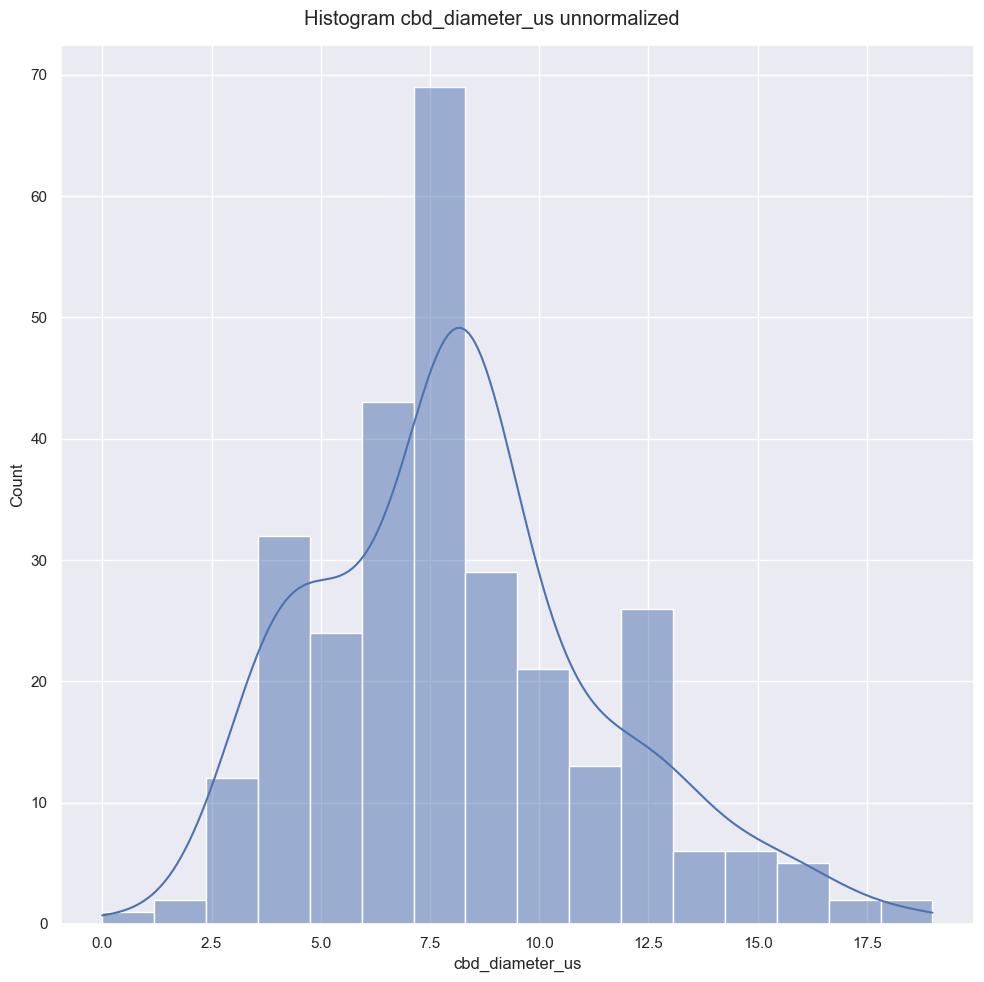
\includegraphics[width=\textwidth]{histogram_cbd_diameter_us_unnormalized}
		\caption{Histograma de atributo \emph{cbd\_diameter\_us} sin normalizar.}
	\end{subfigure}
	\hfill
	\begin{subfigure}[b]{0.4\textwidth}
		\centering
		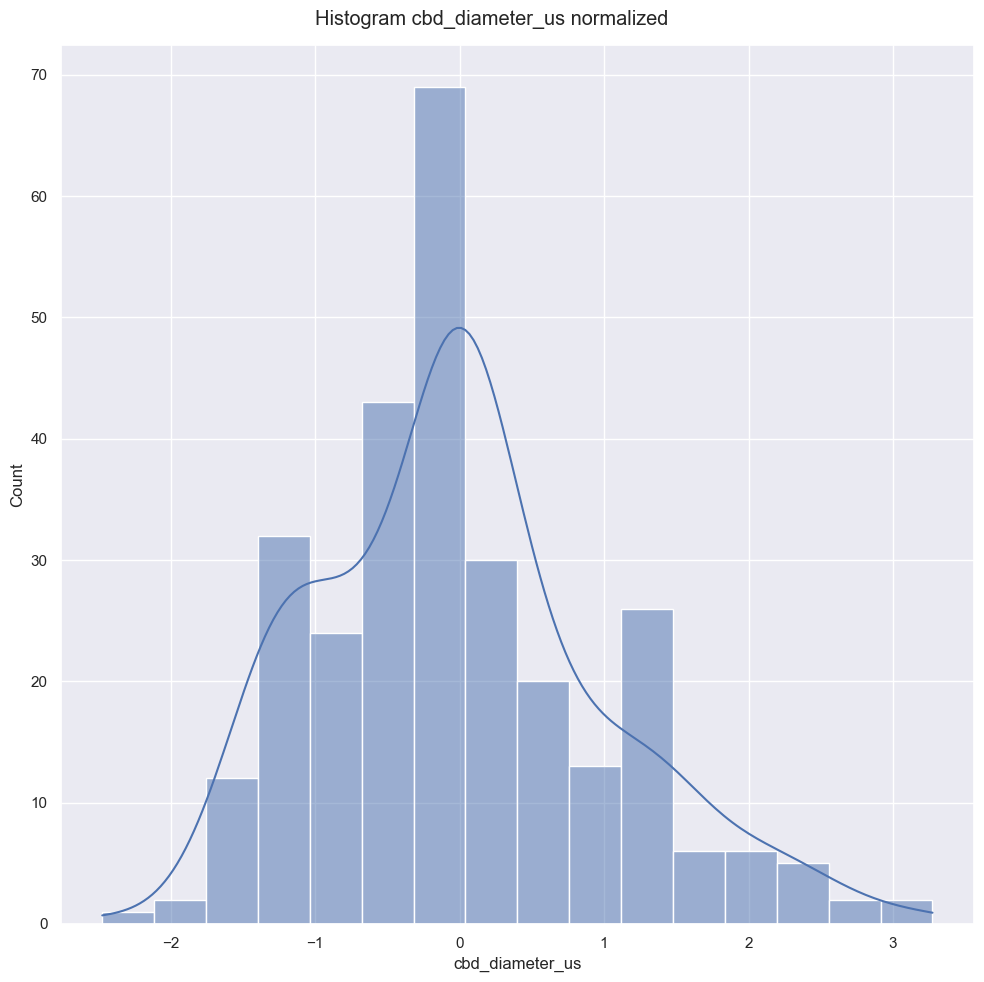
\includegraphics[width=\textwidth]{histogram_cbd_diameter_us_normalized}
		\caption{Histograma de atributo \emph{cbd\_diameter\_us} posterior a normalización.}
	\end{subfigure}
	\caption{Resultados de normalización de atributo \emph{cbd\_diameter\_us}}
	\label{Fig: cbd_diameter_us_NORM}
\end{figure}


\begin{figure}[!htb]
	\centering
	\begin{subfigure}[b]{0.4\textwidth}
		\centering
		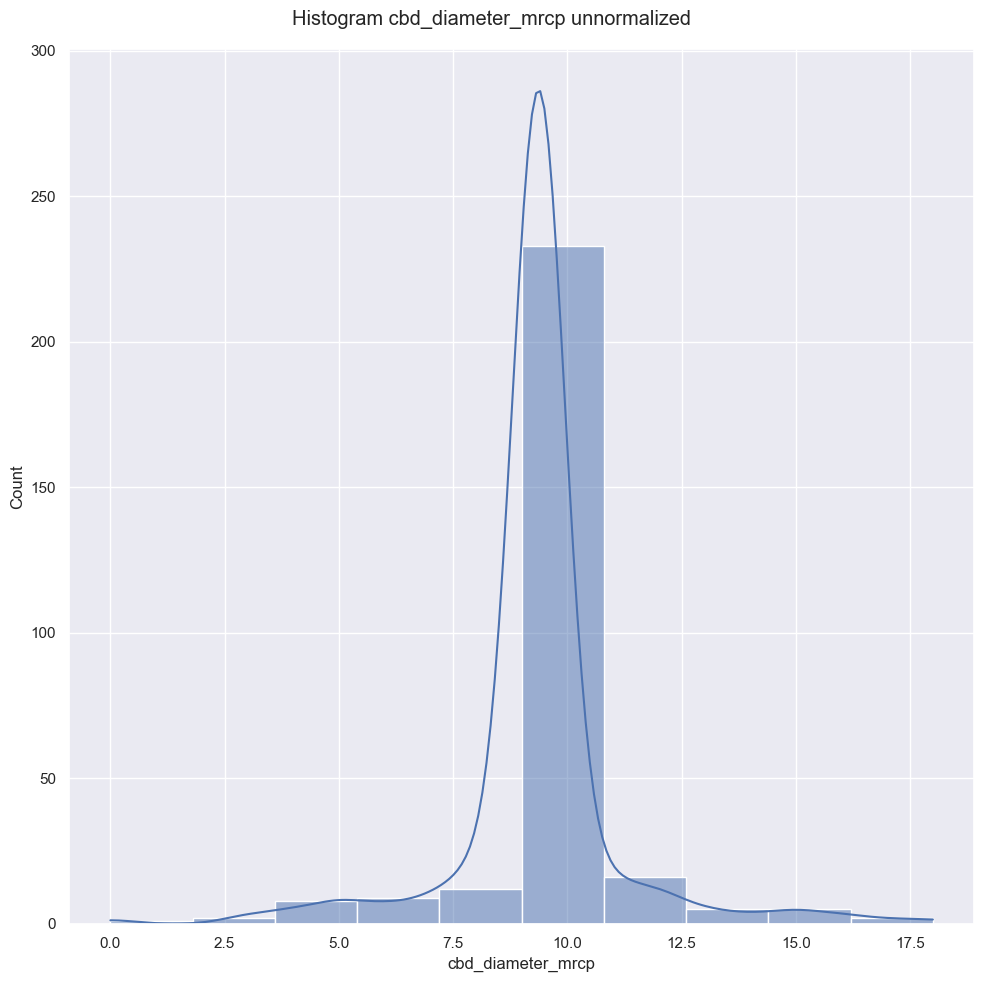
\includegraphics[width=\textwidth]{histogram_cbd_diameter_mrcp_unnormalized}
		\caption{Histograma de atributo \emph{cbd\_diameter\_mrcp} sin normalizar.}
	\end{subfigure}
	\hfill
	\begin{subfigure}[b]{0.4\textwidth}
		\centering
		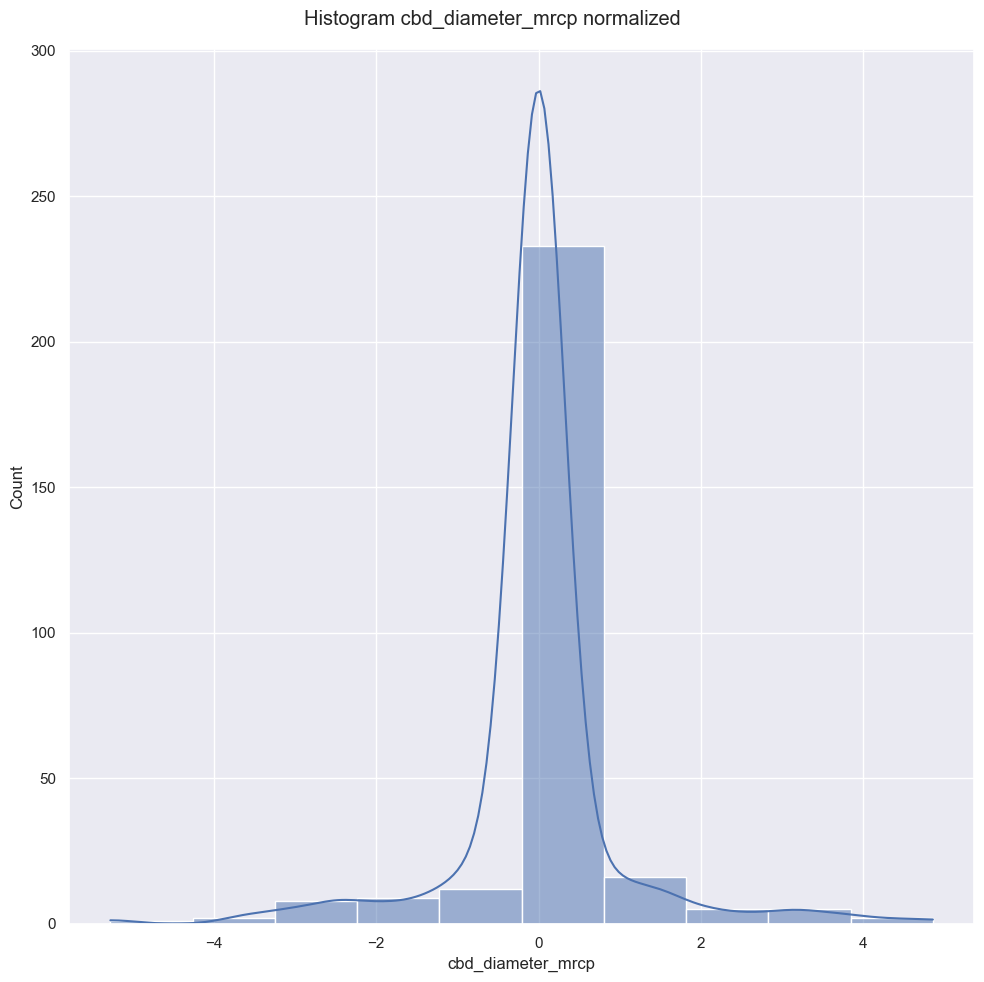
\includegraphics[width=\textwidth]{histogram_cbd_diameter_mrcp_normalized}
		\caption{Histograma de atributo \emph{cbd\_diameter\_mrcp} posterior a normalización.}
	\end{subfigure}
	\caption{Resultados de normalización de atributo \emph{cbd\_diameter\_mrcp}}
	\label{Fig: cbd_diameter_mrcp_NORM}
\end{figure}


\begin{figure}[!htb]
	\centering
	\begin{subfigure}[b]{0.4\textwidth}
		\centering
		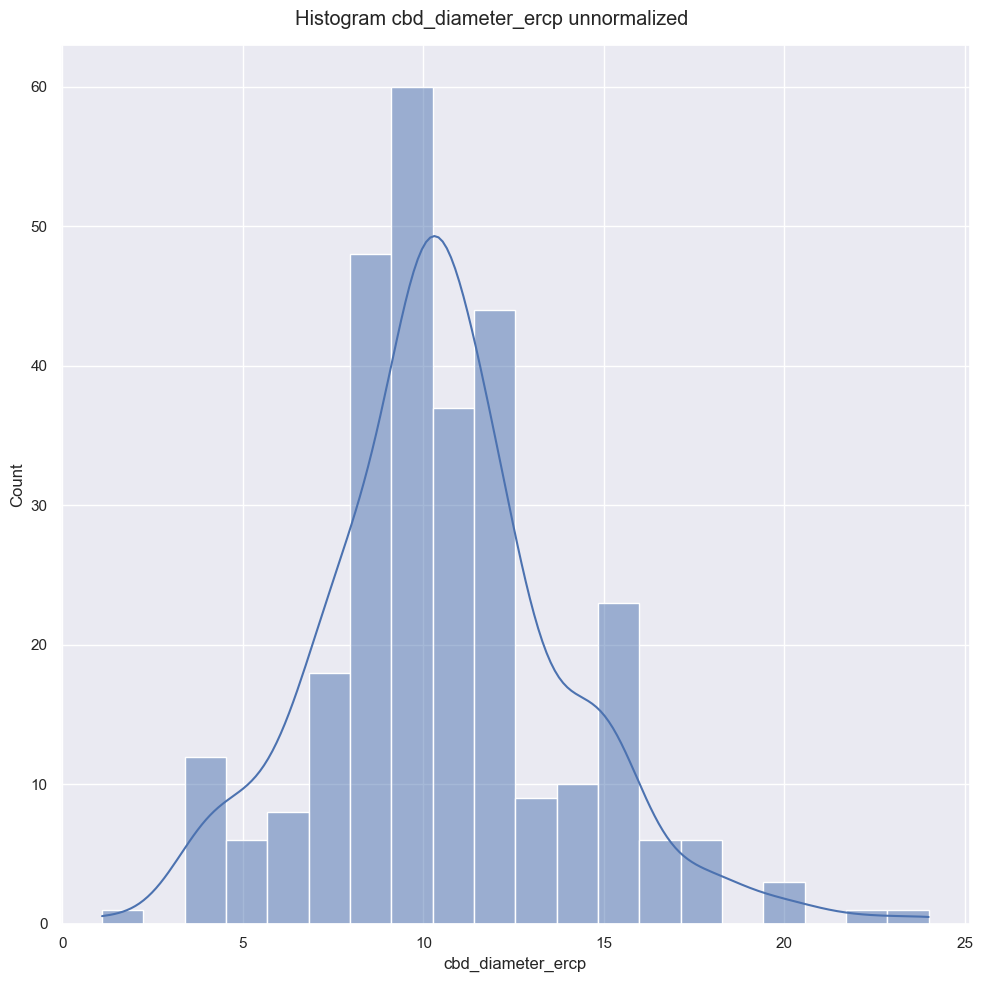
\includegraphics[width=\textwidth]{histogram_cbd_diameter_ercp_unnormalized}
		\caption{Histograma de atributo \emph{cbd\_diameter\_ercp} sin normalizar.}
	\end{subfigure}
	\hfill
	\begin{subfigure}[b]{0.4\textwidth}
		\centering
		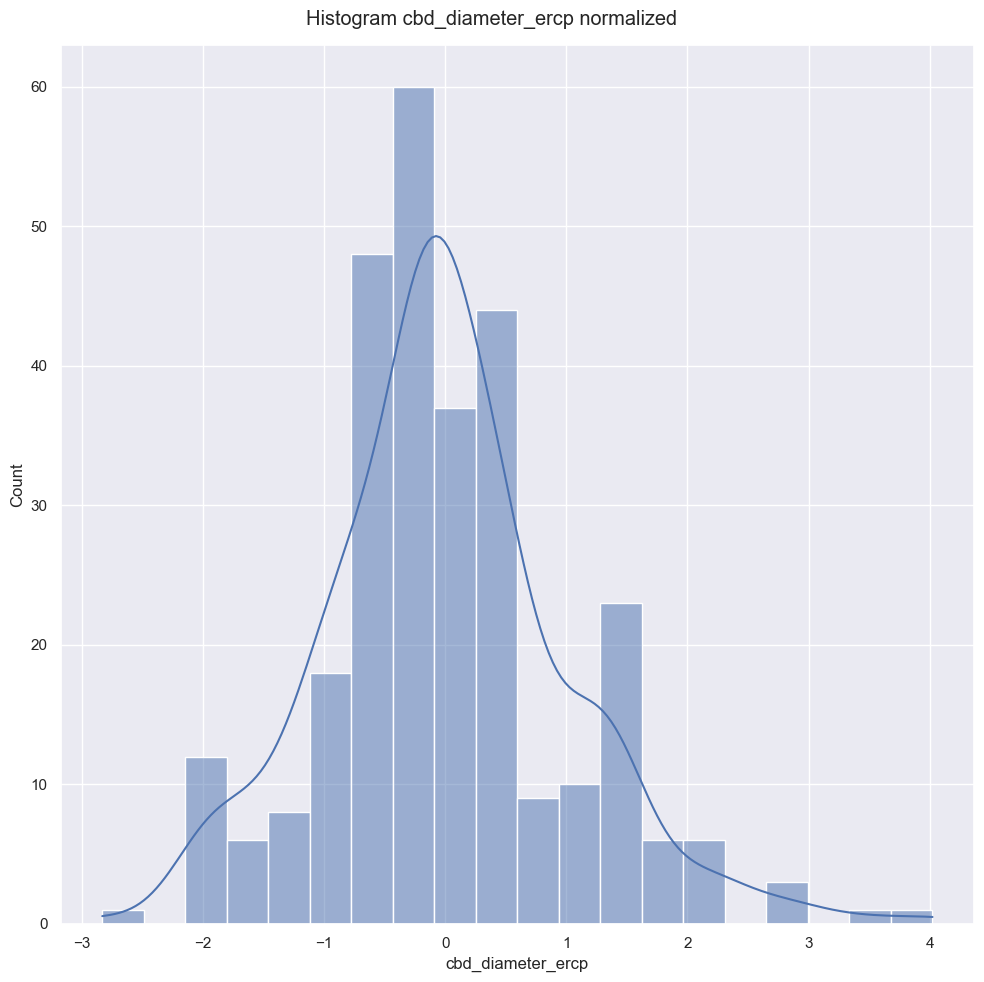
\includegraphics[width=\textwidth]{histogram_cbd_diameter_ercp_normalized}
		\caption{Histograma de atributo \emph{cbd\_diameter\_ercp} posterior a normalización.}
	\end{subfigure}
	\caption{Resultados de normalización de atributo \emph{cbd\_diameter\_mrcp}}
	\label{Fig: cbd_diameter_ercp_NORM}
\end{figure}


\FloatBarrier
\subsubsection{Normalización L1}
La Figuras \ref{Fig: pyobilia_ercp_NORM} - \ref{Fig: stone_shape_ercp_NORM} muestran los resultados de normalización de los atributos elegidos para el método L1.

\begin{figure}[!htb]
	\centering
	\begin{subfigure}[b]{0.4\textwidth}
		\centering
		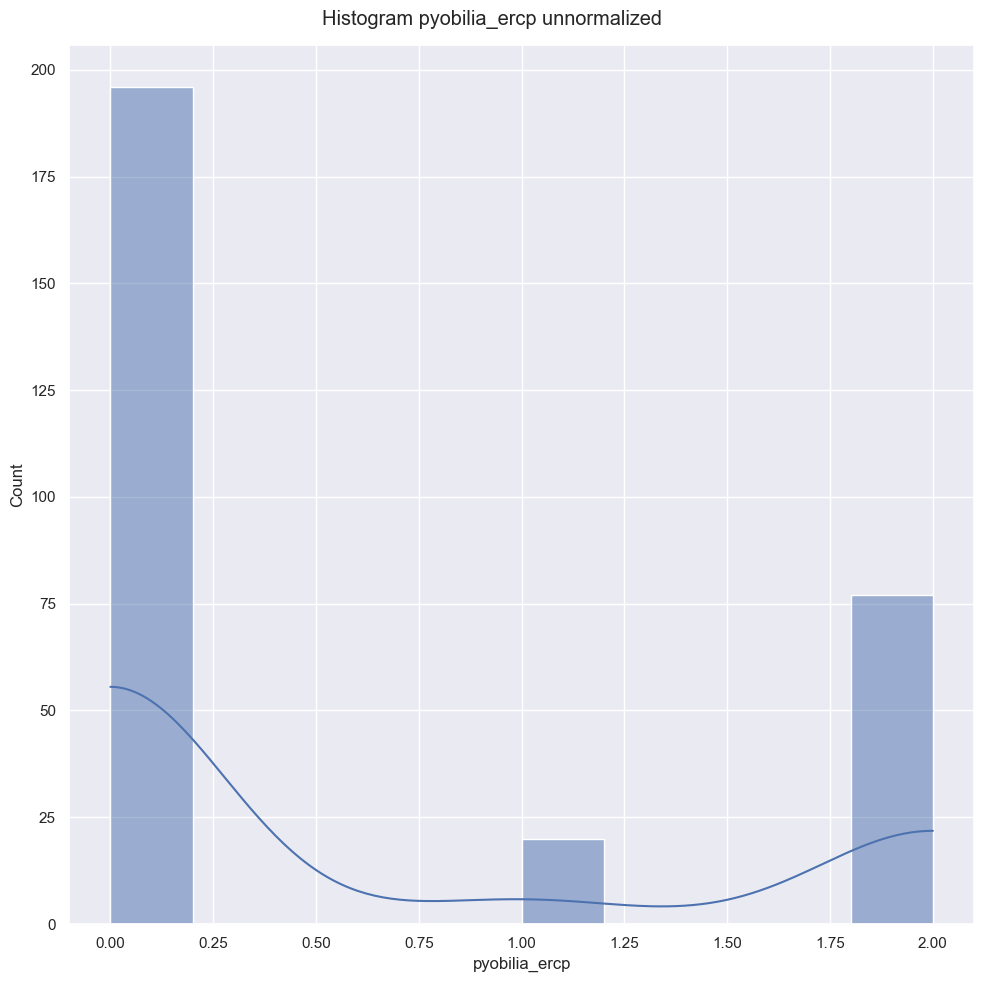
\includegraphics[width=\textwidth]{histogram_pyobilia_ercp_unnormalized}
		\caption{Histograma de atributo \emph{pyobilia\_ercp} sin normalizar.}
	\end{subfigure}
	\hfill
	\begin{subfigure}[b]{0.4\textwidth}
		\centering
		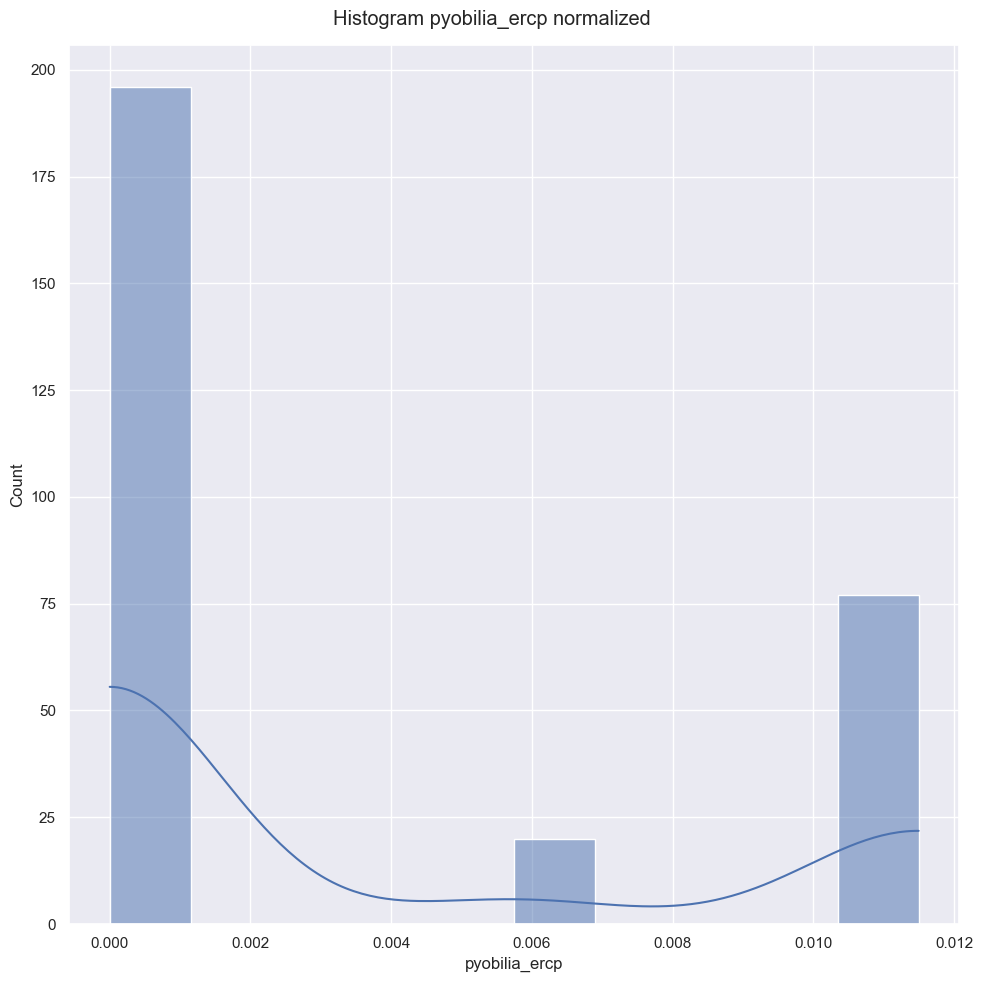
\includegraphics[width=\textwidth]{histogram_pyobilia_ercp_normalized}
		\caption{Histograma de atributo \emph{pyobilia\_ercp} posterior a normalización.}
	\end{subfigure}
	\caption{Resultados de normalización de atributo \emph{pyobilia\_ercp}}
	\label{Fig: pyobilia_ercp_NORM}
\end{figure}


\begin{figure}[!htb]
	\centering
	\begin{subfigure}[b]{0.4\textwidth}
		\centering
		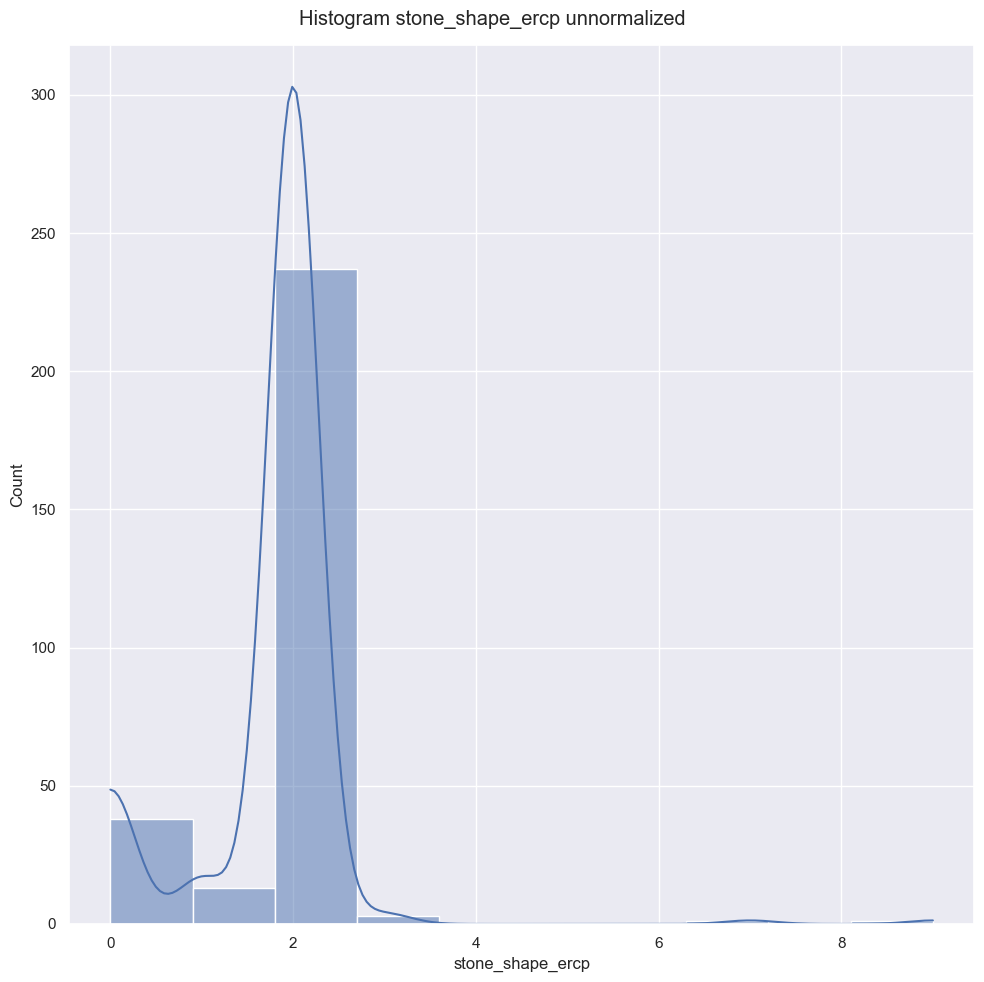
\includegraphics[width=\textwidth]{histogram_stone_shape_ercp_unnormalized}
		\caption{Histograma de atributo \emph{stone\_shape\_ercp} sin normalizar.}
	\end{subfigure}
	\hfill
	\begin{subfigure}[b]{0.4\textwidth}
		\centering
		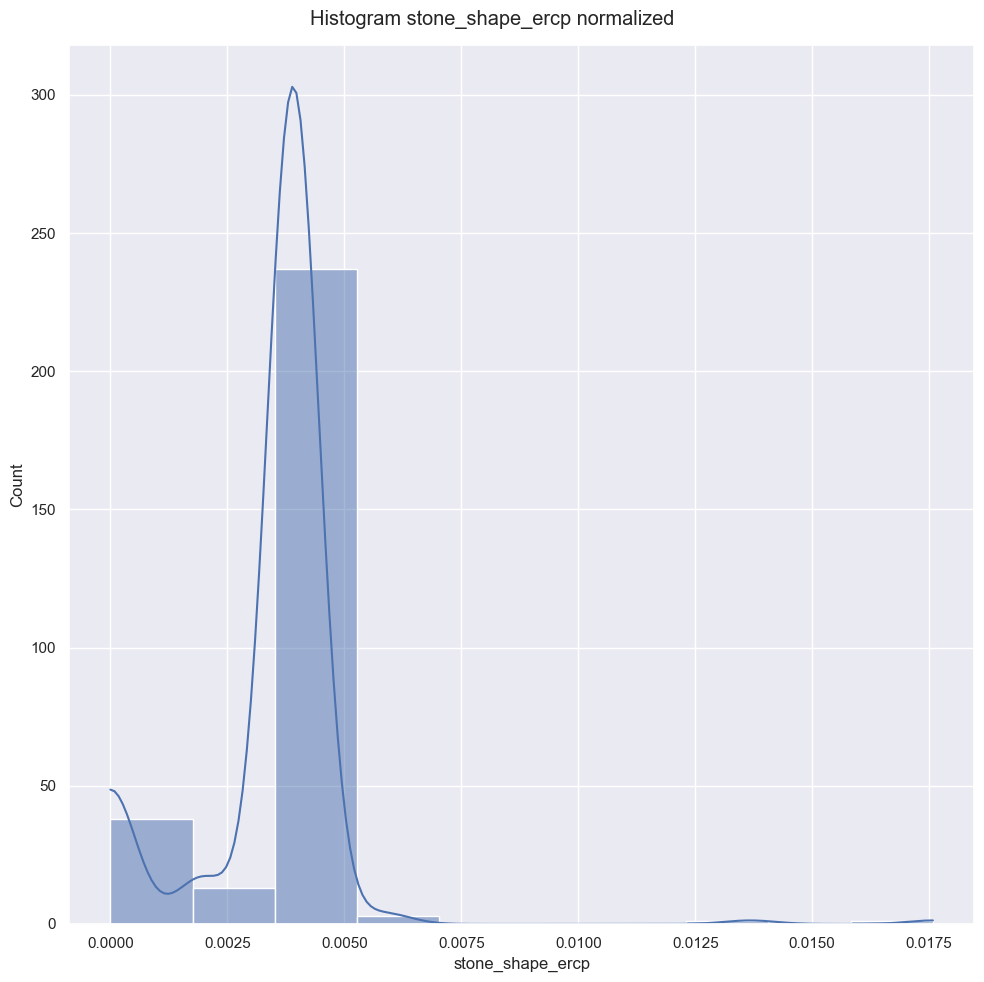
\includegraphics[width=\textwidth]{histogram_stone_shape_ercp_normalized}
		\caption{Histograma de atributo \emph{stone\_shape\_ercp} posterior a normalización.}
	\end{subfigure}
	\caption{Resultados de normalización de atributo \emph{stone\_shape\_ercp}}
	\label{Fig: stone_shape_ercp_NORM}
\end{figure}


\begin{figure}[!htb]
	\centering
	\begin{subfigure}[b]{0.4\textwidth}
		\centering
		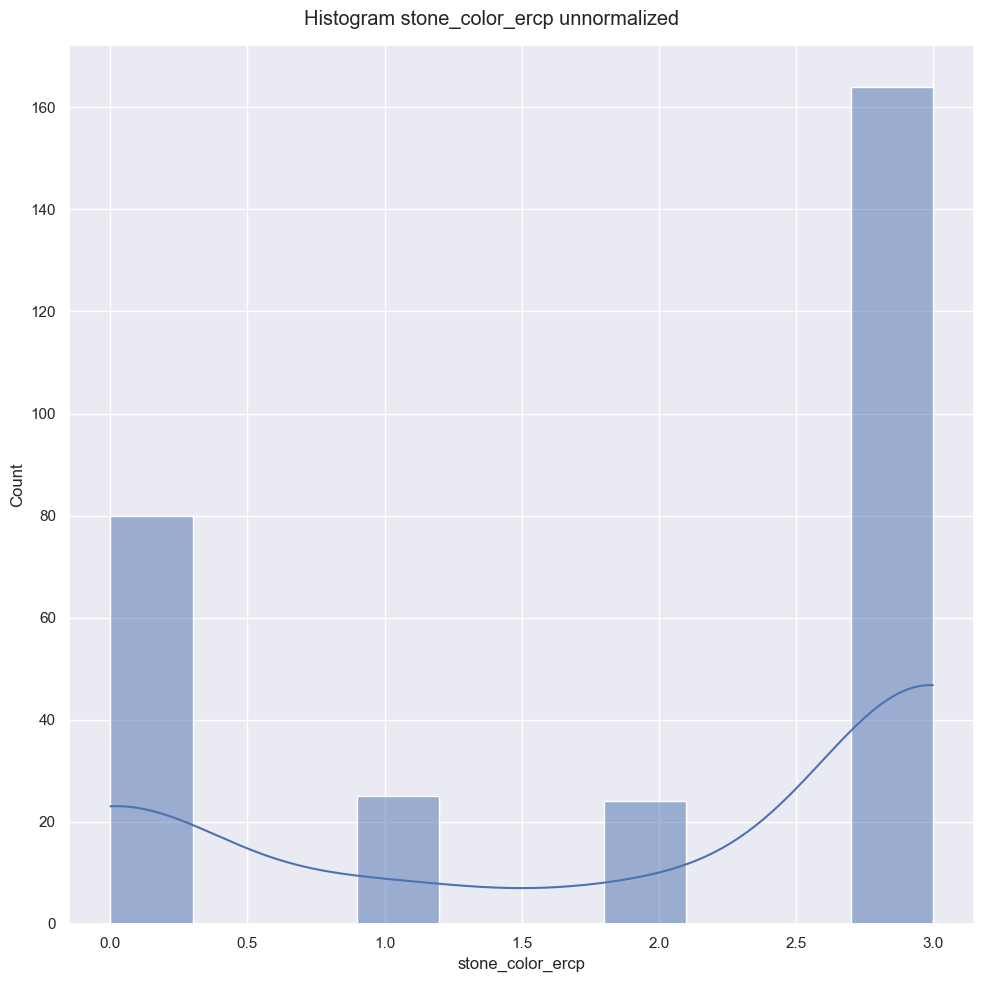
\includegraphics[width=\textwidth]{histogram_stone_color_ercp_unnormalized}
		\caption{Histograma de atributo \emph{stone\_color\_ercp} sin normalizar.}
	\end{subfigure}
	\hfill
	\begin{subfigure}[b]{0.4\textwidth}
		\centering
		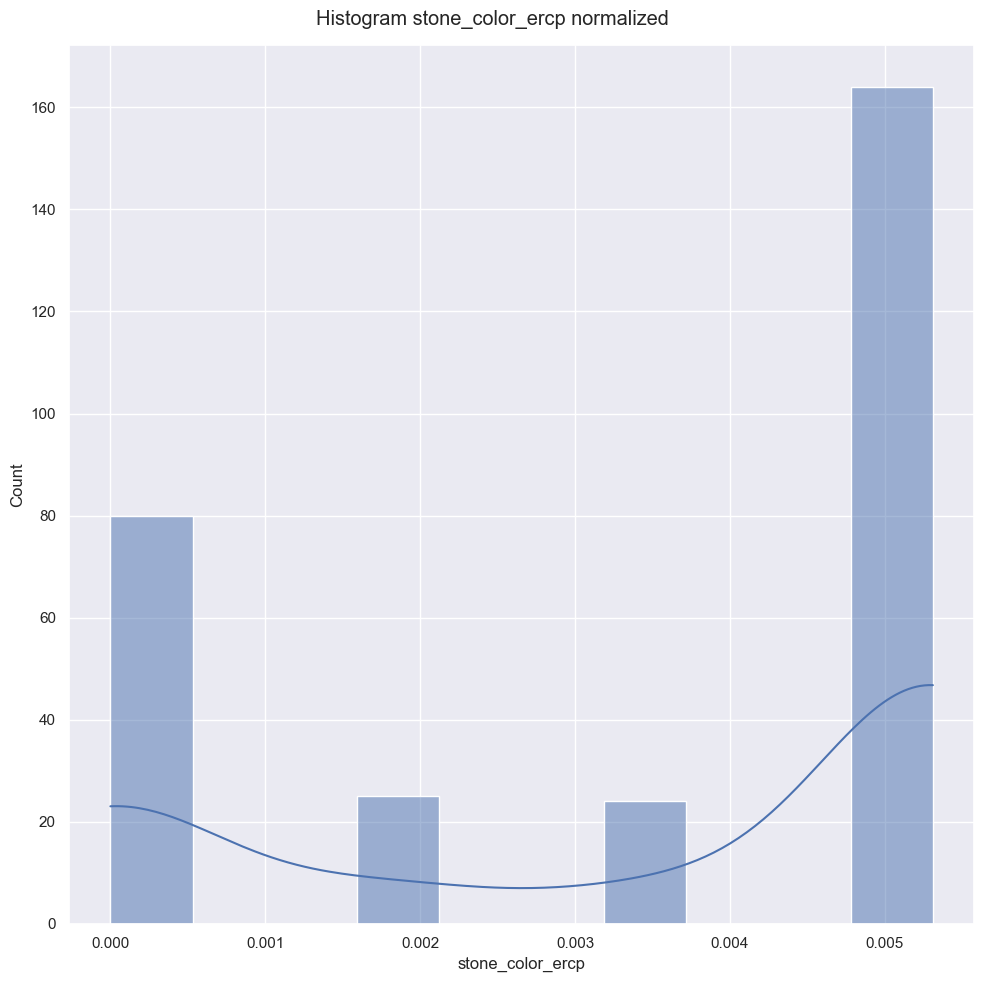
\includegraphics[width=\textwidth]{histogram_stone_color_ercp_normalized}
		\caption{Histograma de atributo \emph{stone\_color\_ercp} posterior a normalización.}
	\end{subfigure}
	\caption{Resultados de normalización de atributo \emph{stone\_shape\_ercp}}
	\label{Fig: stone_shape_ercp_NORM}
\end{figure}

%%%%%%%%%%

\FloatBarrier
\hfill \break
\subsection{Balance de clases con datos sintéticos}
La Figura \ref{Fig: original-class} muestra la distribución de clases original del conjunto de datos.

\begin{figure}[!htb]
	\centering
	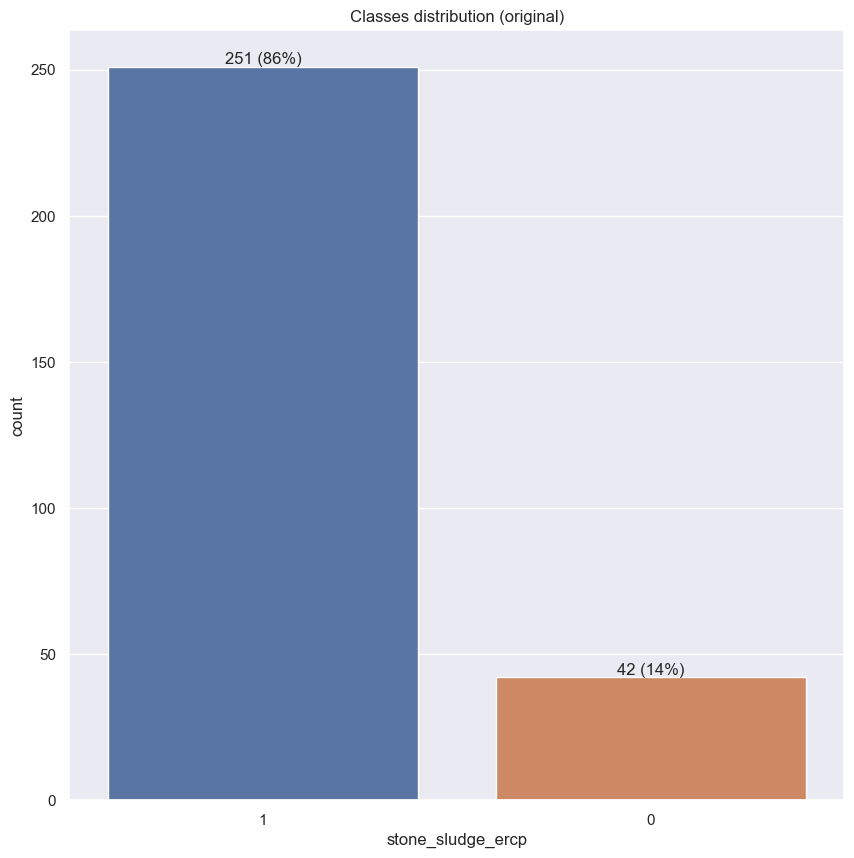
\includegraphics[width=0.7\textwidth]{classes_distribution_original}
	\caption{Distribución de clases en el conjunto de datos original}
	\label{Fig: original-class}
\end{figure}

\FloatBarrier
\subsubsection{Método de ruleta}
La Figura \ref{Fig: roulette-class} muestra la distribución de clases resultante de aplicar el método de ruleta. La Tabla \ref{Tab: Ruleta-std} muestra una comparación entre la desviación estándar de los atributos de la base datos original y los datos obtenidos tras aplicar el método ruleta. Por otro lado, la Figura \ref{Fig: roulette-hist} muestra un ejemplo de la distribución de los datos resultantes del método ruleta.

\begin{figure}[!htb]
	\centering
	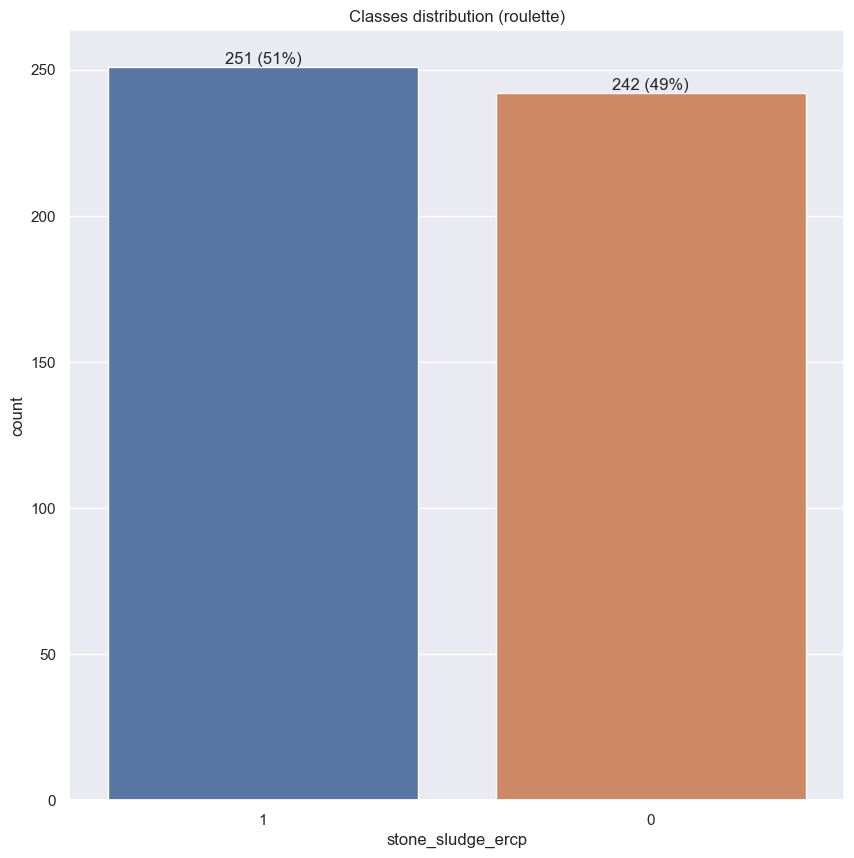
\includegraphics[width=0.7\textwidth]{classes_distribution_roulette}
	\caption{Distribución de clases en el conjunto de datos resultante del método de ruleta}
	\label{Fig: roulette-class}
\end{figure}

\begin{table}[!htb]
\centering
\caption{Comparación de los valores de desviación estándar del conjunto de datos original y posterior al balance de clases por le método de la ruleta.}
\label{Tab: Ruleta-std}
\begin{tabular}{|l|ll|}
\hline
\multicolumn{1}{|c|}{\multirow{2}{*}{\textbf{Atributo}}} & \multicolumn{2}{c|}{\textbf{$\sigma$}}                                           \\ \cline{2-3} 
\multicolumn{1}{|c|}{}                                   & \multicolumn{1}{c|}{\textbf{Original}} & \multicolumn{1}{c|}{\textbf{Ruleta}} \\ \hline
age\_at\_ercp                                            & \multicolumn{1}{l|}{17.81}             & 17.49                                \\ \hline
gender                                                   & \multicolumn{1}{l|}{0.48}              & 0.49                                 \\ \hline
race                                                     & \multicolumn{1}{l|}{1.19}              & 1.25                                 \\ \hline
bmi                                                      & \multicolumn{1}{l|}{7.47}              & 1.15                                 \\ \hline
parity                                                   & \multicolumn{1}{l|}{1.34}              & 0.46                                 \\ \hline
dm                                                       & \multicolumn{1}{l|}{0.36}              & 0.41                                 \\ \hline
ibd                                                      & \multicolumn{1}{l|}{0.05}              & 0.45                                 \\ \hline
cirrhosis                                                & \multicolumn{1}{l|}{0.18}              & 0.21                                 \\ \hline
peak\_bili                                               & \multicolumn{1}{l|}{19.73}             & 29.91                                \\ \hline
stones\_on\_bd                                           & \multicolumn{1}{l|}{1.10}              & 1.14                                 \\ \hline
cbd\_diameter\_us                                        & \multicolumn{1}{l|}{3.31}              & 3.27                                 \\ \hline
cbd\_diameter\_mrcp                                      & \multicolumn{1}{l|}{1.77}              & 1.67                                 \\ \hline
cbd\_diameter\_ercp                                      & \multicolumn{1}{l|}{3.34}              & 3.37                                 \\ \hline
intraductal\_filling                                     & \multicolumn{1}{l|}{0.94}              & 1.18                                 \\ \hline
cystic\_duct\_filling                                    & \multicolumn{1}{l|}{0.88}              & 0.92                                 \\ \hline
stone\_shape\_ercp                                       & \multicolumn{1}{l|}{0.87}              & 0.85                                 \\ \hline
stone\_color\_ercp                                       & \multicolumn{1}{l|}{1.31}              & 1.17                                 \\ \hline
pyobilia\_ercp                                           & \multicolumn{1}{l|}{0.87}              & 0.87                                 \\ \hline
gallbladder                                              & \multicolumn{1}{l|}{0.50}              & 0.53                                 \\ \hline
stone\_sludge\_ercp                                      & \multicolumn{1}{l|}{0.35}              & 0.50                                 \\ \hline
\end{tabular}
\end{table}

\begin{figure}[!htb]
	\centering
	\begin{subfigure}[b]{0.4\textwidth}
		\centering
		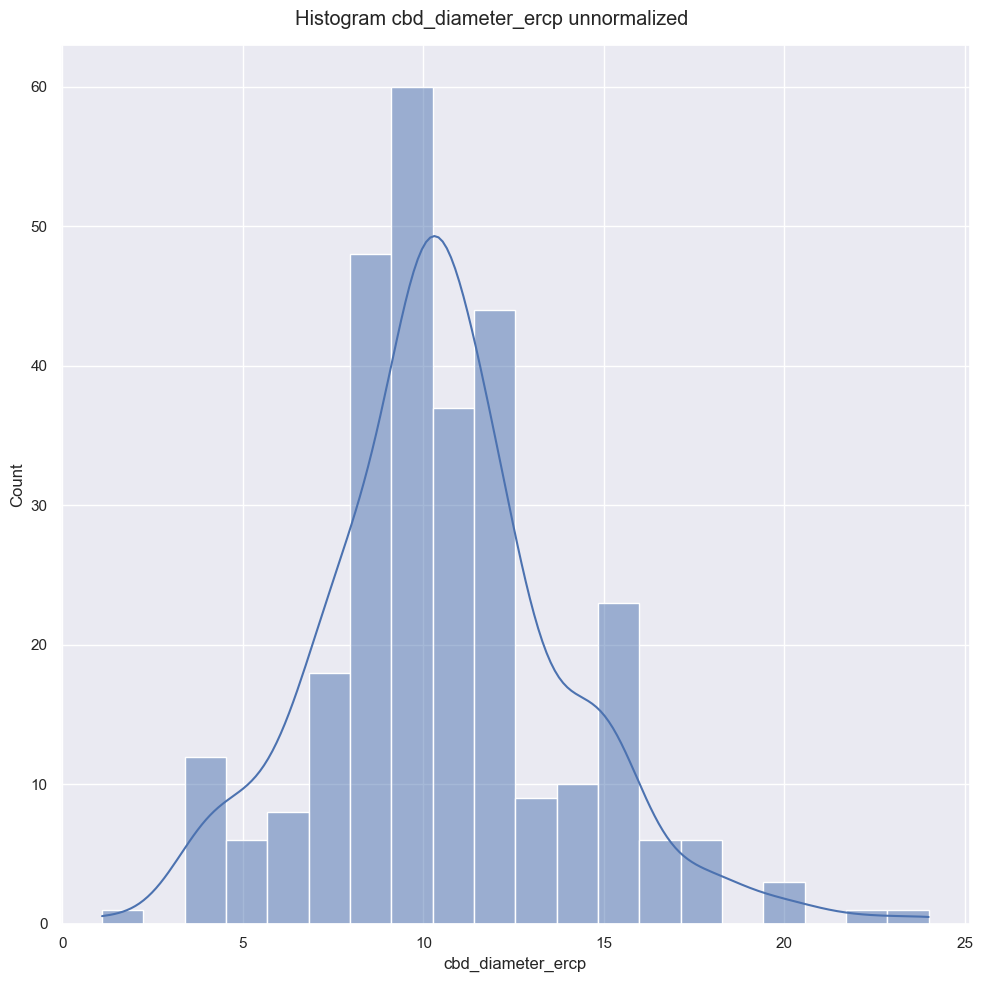
\includegraphics[width=\textwidth]{histogram_cbd_diameter_ercp_unnormalized}
		\caption{Histograma de atributo \emph{cbd\_diameter\_ercp} original.}
	\end{subfigure}
	\hfill
	\begin{subfigure}[b]{0.4\textwidth}
		\centering
		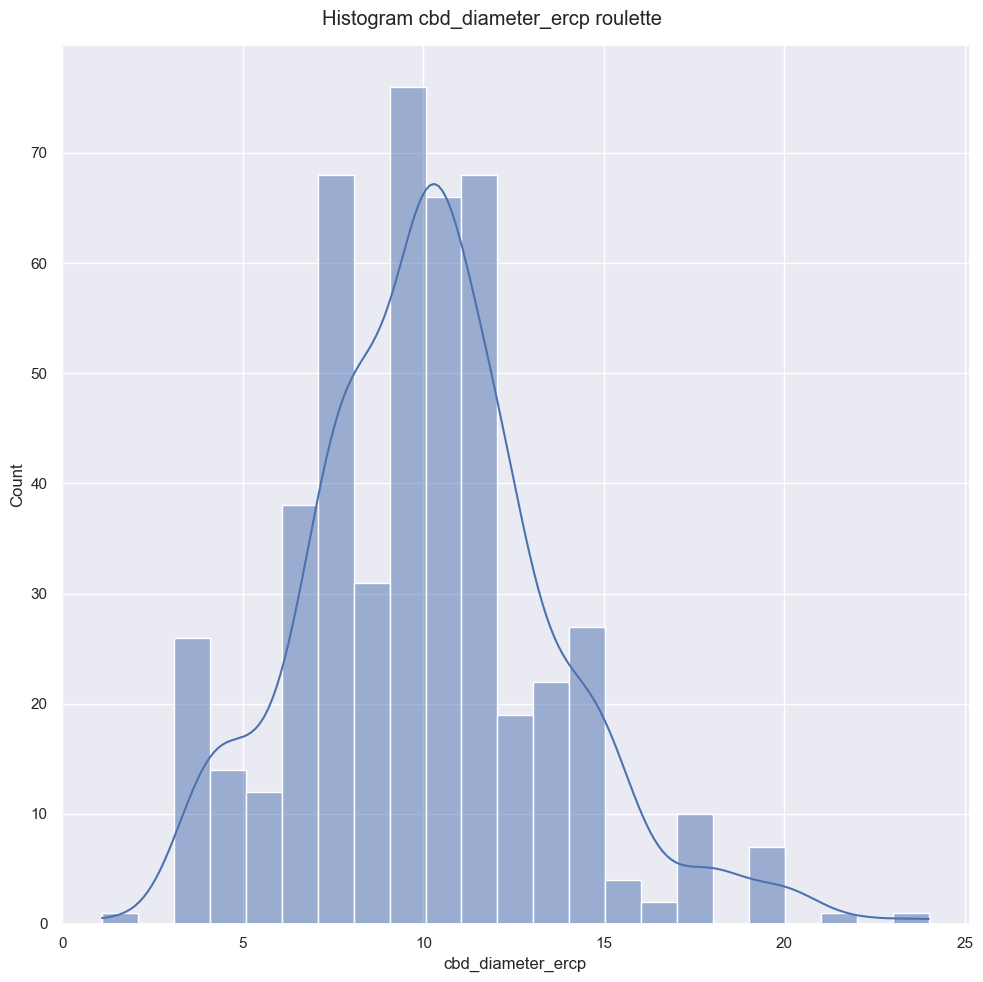
\includegraphics[width=\textwidth]{histogram_cbd_diameter_ercp_roulette}
		\caption{Histograma de atributo \emph{cbd\_diameter\_ercp} posterior a método de ruleta.}
	\end{subfigure}
	\caption{Resultados de datos sintéticos mediante el método ruleta}
	\label{Fig: roulette-hist}
\end{figure}


\FloatBarrier
\subsubsection{SMOTE}
La Figura \ref{Fig: SMOTE-class} muestra la distribución de clases resultante de aplicar el método SMOTE. La Tabla \ref{Tab: SMOTE-std} muestra una comparación entre la desviación estándar de los atributos de la base datos original y los datos obtenidos tras aplicar el método SMOTE. Por otro lado, la Figura \ref{Fig: smote-hist} muestra un ejemplo de la distribución de los datos resultantes del método SMOTE.

\begin{figure}[!htb]
	\centering
	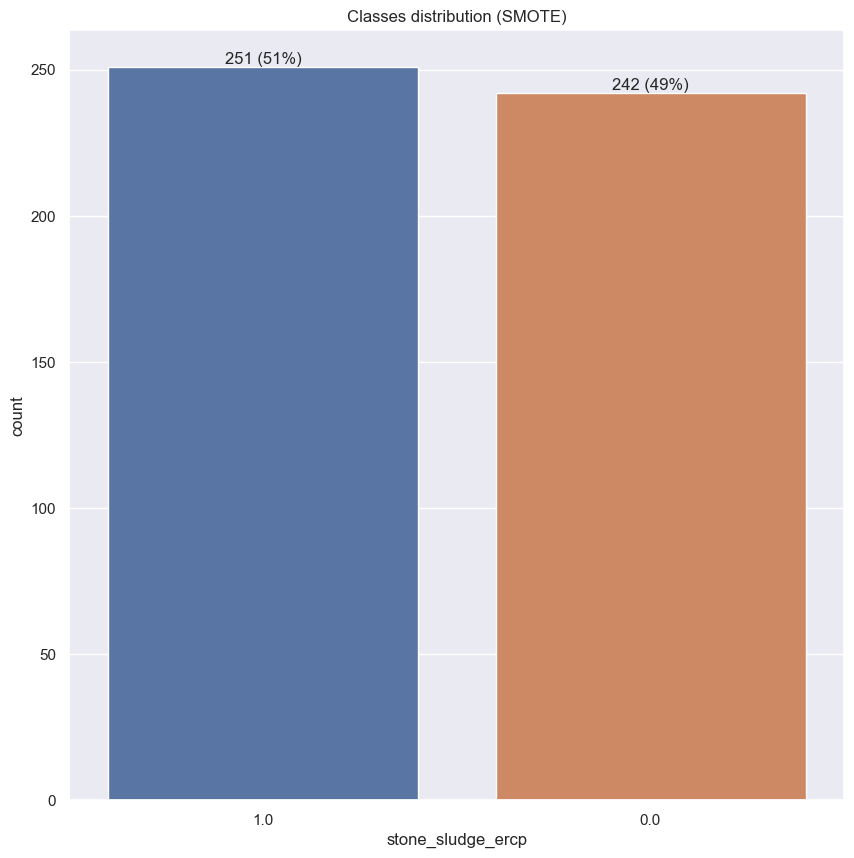
\includegraphics[width=0.7\textwidth]{classes_distribution_smote}
	\caption{Distribución de clases en el conjunto de datos resultante del método SMOTE}
	\label{Fig: SMOTE-class}
\end{figure}

\begin{table}[!htb]
\centering
\caption{Comparación de los valores de desviación estándar del conjunto de datos original y posterior al balance de clases por el método SMOTE.}
\label{Tab: SMOTE-std}
\begin{tabular}{|l|ll|}
\hline
\multicolumn{1}{|c|}{\multirow{2}{*}{\textbf{Atributo}}} & \multicolumn{2}{c|}{\textbf{$\sigma$}}                                           \\ \cline{2-3} 
\multicolumn{1}{|c|}{}                                   & \multicolumn{1}{c|}{\textbf{Original}} & \multicolumn{1}{c|}{\textbf{SMOTE}} \\ \hline
age\_at\_ercp                                            & \multicolumn{1}{l|}{17.81}             & 17.07                                \\ \hline
gender                                                   & \multicolumn{1}{l|}{0.48}              & 0.46                                 \\ \hline
race                                                     & \multicolumn{1}{l|}{1.19}              & 1.18                                 \\ \hline
bmi                                                      & \multicolumn{1}{l|}{7.47}              & 7.50                                 \\ \hline
parity                                                   & \multicolumn{1}{l|}{1.34}              & 1.15                                 \\ \hline
dm                                                       & \multicolumn{1}{l|}{0.36}              & 0.39                                 \\ \hline
ibd                                                      & \multicolumn{1}{l|}{0.05}              & 0.04                                 \\ \hline
cirrhosis                                                & \multicolumn{1}{l|}{0.18}              & 0.17                                 \\ \hline
peak\_bili                                               & \multicolumn{1}{l|}{19.73}             & 25.85                                \\ \hline
stones\_on\_bd                                           & \multicolumn{1}{l|}{1.10}              & 1.09                                 \\ \hline
cbd\_diameter\_us                                        & \multicolumn{1}{l|}{3.31}              & 3.14                                 \\ \hline
cbd\_diameter\_mrcp                                      & \multicolumn{1}{l|}{1.77}              & 1.54                                 \\ \hline
cbd\_diameter\_ercp                                      & \multicolumn{1}{l|}{3.34}              & 3.37                                 \\ \hline
intraductal\_filling                                     & \multicolumn{1}{l|}{0.94}              & 1.11                                 \\ \hline
cystic\_duct\_filling                                    & \multicolumn{1}{l|}{0.88}              & 0.87                                 \\ \hline
stone\_shape\_ercp                                       & \multicolumn{1}{l|}{0.87}              & 0.76                                 \\ \hline
stone\_color\_ercp                                       & \multicolumn{1}{l|}{1.31}              & 1.15                                 \\ \hline
pyobilia\_ercp                                           & \multicolumn{1}{l|}{0.87}              & 0.84                                 \\ \hline
gallbladder                                              & \multicolumn{1}{l|}{0.50}              & 0.48                                 \\ \hline
stone\_sludge\_ercp                                      & \multicolumn{1}{l|}{0.35}              & 0.50                                 \\ \hline
\end{tabular}
\end{table}

\begin{figure}[!htb]
	\centering
	\begin{subfigure}[b]{0.4\textwidth}
		\centering
		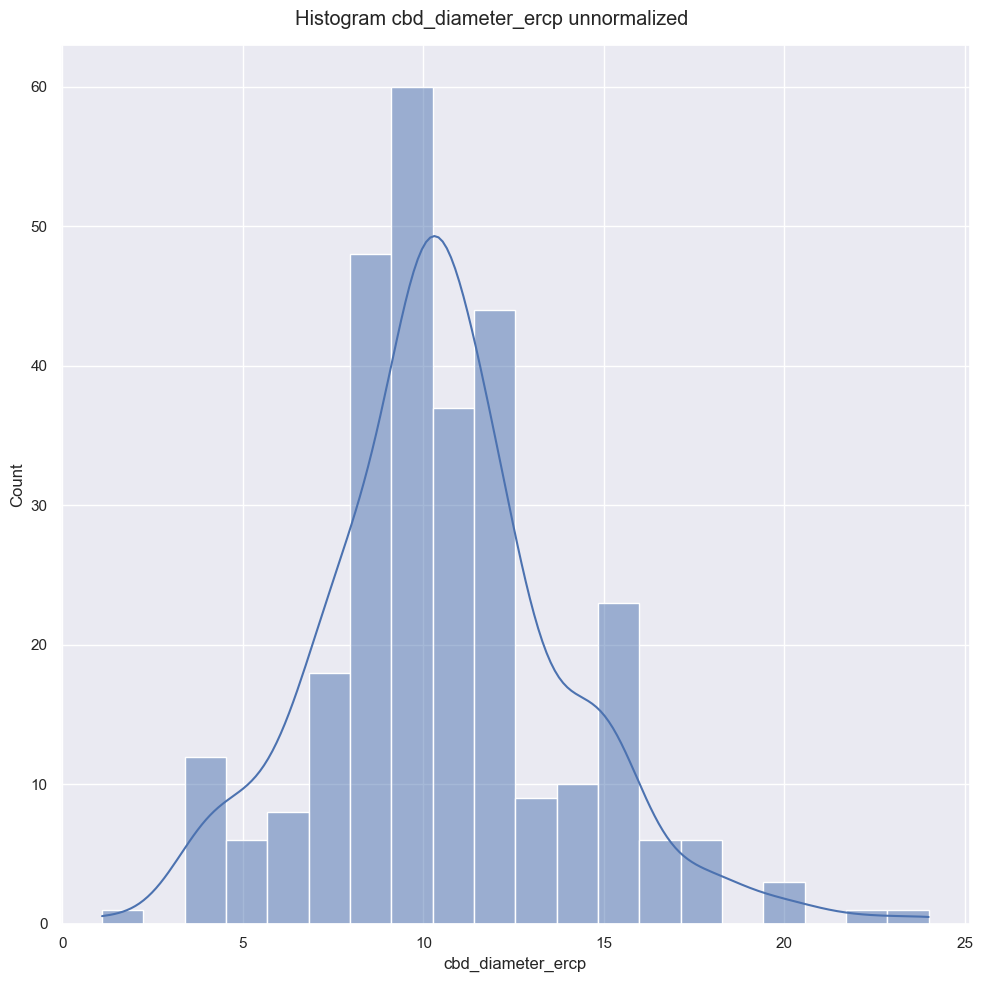
\includegraphics[width=\textwidth]{histogram_cbd_diameter_ercp_unnormalized}
		\caption{Histograma de atributo \emph{cbd\_diameter\_ercp} original.}
	\end{subfigure}
	\hfill
	\begin{subfigure}[b]{0.4\textwidth}
		\centering
		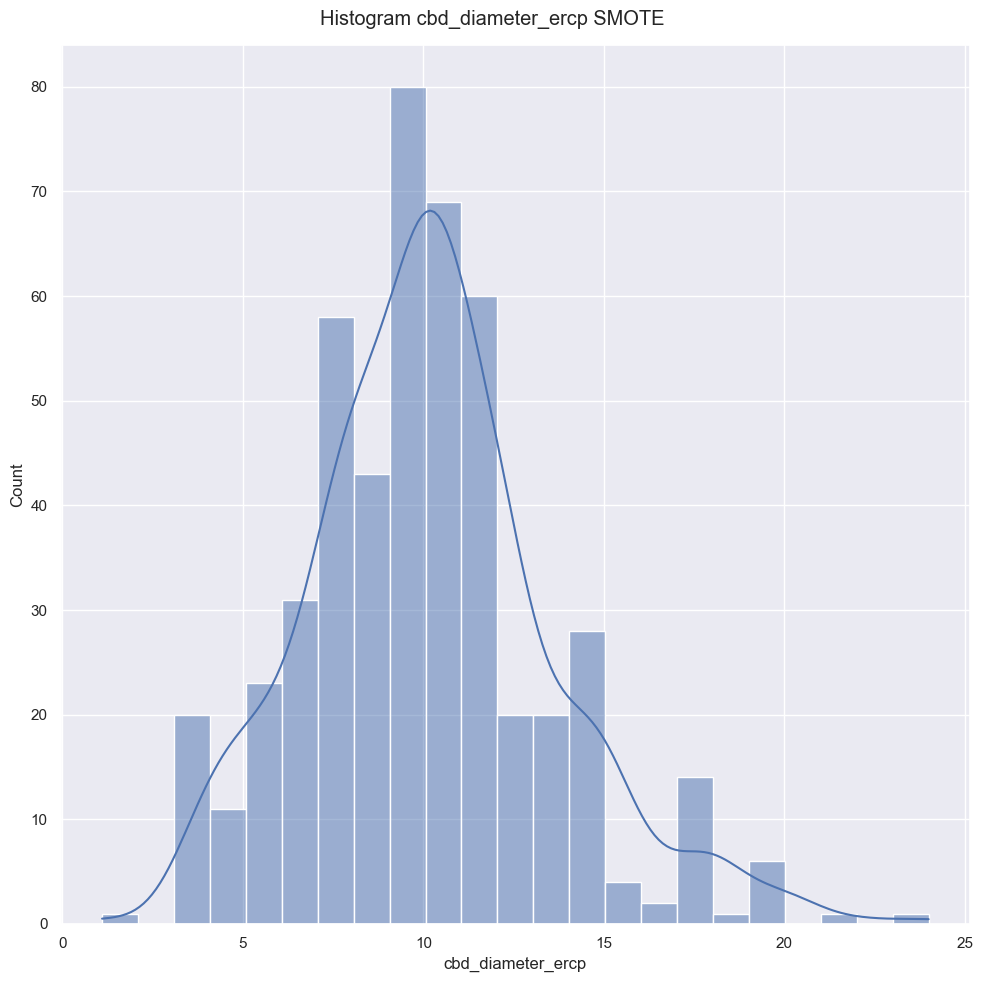
\includegraphics[width=\textwidth]{histogram_cbd_diameter_ercp_smote}
		\caption{Histograma de atributo \emph{cbd\_diameter\_ercp} posterior a método SMOTE.}
	\end{subfigure}
	\caption{Resultados de datos sintéticos mediante el método SMOTE}
	\label{Fig: smote-hist}
\end{figure}
